\chapter{Trigonometry}

In the first half of this chapter the three trigonometric functions (sine, cosine and tangent) will be viewed as functions of angles. The second half of the chapter will approach trigonometry as functions of real numbers.

\section{The Measurement of Angles}
It should come as no surprise that the convention for measuring angles should be the same as for measuring
the distance around the perimeter of the unit circle.. An angle is measured in degrees and is the amount of
rotation between two rays about a vertex. If the vertex is placed at the point $\left (0 ,0\right )$ and one ray is placed along the positive $x$-axis then we let the second ray go through the point $P (x ,y)$ on the unit circle so that the relationship between the angle and $t$ (see chapter $2$) can be established. The convention is that the positive direction for measuring
angles is anticlockwise and the negative direction for measuring angles is clockwise. You will be aware that
one complete cycle measures 360$\mbox{{\ensuremath{{}^\circ}}}$. One degree therefore is $\frac{1}{360}$\ of one complete cycle. In this subject the
word revolution is often used instead of cycle. Other terms with which you might be familiar are "a quarter
turn" for $90 \mbox{{\ensuremath{{}^\circ}}}$ and "a half turn" for $180 \mbox{{\ensuremath{{}^\circ}}}$. 

If you draw a unit circle (centre $\left (0 ,0\right )$ radius $1$) then you can draw the ray through any terminal point and show the relationship between $t$ and the angle at the vertex $\left (0 ,0\right )$. 

Definition: If the unit circle is drawn and the distance $t$ is measured around the perimeter from $\left (1 ,0\right )$ to the point $P (x ,y)$ then we say the angle is measured as $t$ \emph{radians}. 

The abbreviation for radians is $\mbox{rad}$. This abbreviation will be used in the examples.
Some books uses the term "angles in standard position" to describe this situation. We
will not define this term unless it is unavoidable and will stick to 'rad'.

Using the language of geometry, the unit circle is cut by two rays one through the points $\left (0 ,0\right )$ and $\left (1 ,0\right )$ and the other through the points $\left (0 ,0\right )$ and $P \left (x ,y\right )$.  
\columnsep =30pt
\begin {multicols}{2}
   
\setlength\fboxrule{0in}\setlength\fboxsep{0.2in}\fcolorbox[HTML]{000000}{FFFFFF}{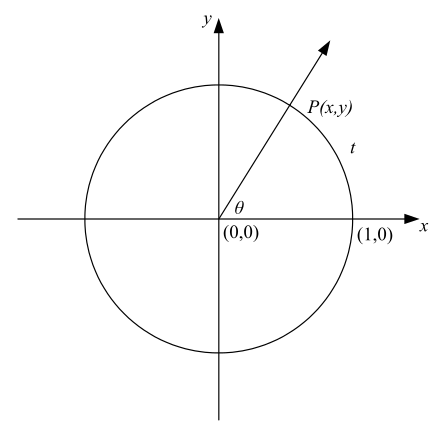
\includegraphics[ width=2.469in, height=2.4275in,]{L4SZ281A}
}

$t$ is referred to as "the length of the arc". The
angle $\theta $ between the two rays is referred to as "the angle \emph{subtended} at the point $\left (0 ,0\right )$". 

We will often leave out the word "subtended"
however this is because it is implied and we really should have used it. 


%TCIMACRO{\TeXButton{End Two Columns}{\end {multicols}}}%
%BeginExpansion
\end {multicols}
%EndExpansion


We can say therefore that the angle measured in radians is related to the same angle measured in degrees. the
relationship between these two measures must be understood and must be able to be derived. 

\subsection{Relationship between Degrees and Radians}
One complete revolution is 360$\mbox{{\ensuremath{{}^\circ}}}$ if the angle is measured in degrees and $2 \pi $ if the angle is measured in radians. So
\begin{align*}2 \pi \text{}\mbox{rad} &  =  360 \mbox{{\ensuremath{{}^\circ}}} \\
\text{or\  \ }\pi \text{}\mbox{rad} &  =  180 \mbox{{\ensuremath{{}^\circ}}}\end{align*}

You should derive this formula whenever you are asked to convert degrees to radians or radians
to degrees 

\subsubsection{Example}
(a) Convert 36$\mbox{{\ensuremath{{}^\circ}}}$ to radians 

(b) Convert $\frac{\pi }{3}$ $\mbox{rad}$ to degrees 

(c) Convert $1$ $\mbox{rad}$ to degrees 

(a)
\begin{align*}180 \mbox{{\ensuremath{{}^\circ}}} &  =  \pi \text{}\mbox{rad} \\
1 \mbox{{\ensuremath{{}^\circ}}} &  =  \frac{\pi }{180}\text{}\mbox{rad} \\
36 \mbox{{\ensuremath{{}^\circ}}} &  =  \frac{\pi }{180} \times 36 =\frac{\pi }{5}\text{}\mbox{rad}\end{align*}

(b)
\begin{align*}\pi  \mbox{rad} &  =  180 \mbox{{\ensuremath{{}^\circ}}} \\
\frac{\pi }{3} \mbox{rad} &  = \frac{180 \mbox{{\ensuremath{{}^\circ}}}}{3} =60 \mbox{{\ensuremath{{}^\circ}}}\end{align*}

(c)
\begin{align*}\pi  \mbox{rad} &  =  180 \mbox{{\ensuremath{{}^\circ}}} \\
1 \mbox{rad} &  =  \frac{180 \mbox{{\ensuremath{{}^\circ}}}}{\pi } \\
 &  \approx   57.29577951 \mbox{{\ensuremath{{}^\circ}}} \\
 &  \approx   57.3 \mbox{{\ensuremath{{}^\circ}}}\end{align*}

Note the similarity between the answers to (b) and (c). This
is because $\frac{\pi }{3} =1.047197551$ so you would expect the values in degrees to be similar. 



With this terminology we leave out the word measured when we talk about measuring angles. We
say "the angle is $60 \mbox{{\ensuremath{{}^\circ}}}$" when we mean it has been measured as $60 \mbox{{\ensuremath{{}^\circ}}}$ or "the angle is $\frac{\pi }{3}$" to mean it has been measured as $\frac{\pi }{3}$ $\mbox{rad}$. Notice we always put in the degree symbol and
often omit the units when the angle is measured in radians. Should units be omitted assume the angle is measured
in radians. We often use the Greek symbol $\theta $\ for the angle subtended at the centre of the unit circle so $\theta  =60 \mbox{{\ensuremath{{}^\circ}}}$ or $\theta  =\frac{\pi }{3}$ are further examples of terminology that is commonly used.

\subsection{Length of a Circular Arc}
Let $\theta $ be the angle subtended at the centre for the ends of an arc of any circle then the fraction of the circumference of the
circle is $\frac{\theta }{2 \pi }$ if $\theta $ is measured in radians and $\frac{\theta }{360 \mbox{{\ensuremath{{}^\circ}}}}$ if $\theta $ is measured in degrees. 

The length of the circumference of any circle whose radius is $r$ is $2 \pi  r$. 

If $\theta $ is measured in radians
\begin{equation*}\text{Length of arc} =\frac{\theta }{2 \pi } \times 2 \pi  r =\theta  r\text{ or }r \theta 
\end{equation*}

If $\theta $ is measured in degrees
\begin{equation*}\text{Length of arc} =\frac{\theta }{360 \mbox{{\ensuremath{{}^\circ}}}} \times 2 \pi  r
\end{equation*}

The simplicity of the first formula shows why working with radians is preferred. 

\subsubsection{Example}
Find the length of an arc that subtends an angle of 45$\mbox{{\ensuremath{{}^\circ}}}$ at the centre of a circle whose radius is 9 $\mbox{cm}\text{.}$ 

Method 1:
\begin{align*}\text{Length of arc} &  =  \frac{\theta }{360 \mbox{{\ensuremath{{}^\circ}}}} \times 2 \pi  r \\
 &  =  \frac{45}{360} \times 2 \pi  \times 9 \\
 &  =  2.25 \pi \text{}\mbox{cm} \\
 &  \approx   7.07\text{}\mbox{cm}\end{align*}

If an exact answer is required you should leave the answer as $2.25 \pi $ $\mbox{cm}$. (Or $\frac{9 \pi }{4}$ $\mbox{cm}\text{.}$) 

Method 2: Change degrees to radians first
\begin{align*}180 \mbox{{\ensuremath{{}^\circ}}} &  =  \pi \text{}\mbox{rad} \\
1 \mbox{{\ensuremath{{}^\circ}}} &  =  \frac{\pi }{180} \\
45 \mbox{{\ensuremath{{}^\circ}}} &  =  \frac{\pi }{180} \times 45 \\
 &  =  \frac{\pi }{4}\end{align*}


\begin{align*}\text{Length of arc} &  =  r \theta  \\
 &  =  9 \times \frac{\pi }{4} =\frac{9 \pi }{4}\text{}\mbox{cm}\end{align*}


\subsection{Area of Circular Sector}
It is assumed you know how to describe and visualise a sector of a circle and that you know that the area of a circle whose radius is $r$ is $\pi  r^{2}$. Continuing the logic above 

If $\theta $ is measured in radians
\begin{equation*}\text{Area of sector} =\frac{\theta }{2 \pi } \times \pi  r^{2} =\frac{1}{2} r^{2} \theta 
\end{equation*}

If $\theta $ is measured in degrees
\begin{equation*}\text{Area of sector} =\frac{\theta }{360 \mbox{{\ensuremath{{}^\circ}}}} \times \pi  r^{2}
\end{equation*}

\subsubsection{Example}
Find the area of a sector with a central angle of 45$\mbox{{\ensuremath{{}^\circ}}}$ for a circle whose radius is 4 $\mbox{cm}$. 

Method 1
\begin{align*}\text{Area of sector} &  =  \frac{45 \mbox{{\ensuremath{{}^\circ}}}}{360 \mbox{{\ensuremath{{}^\circ}}}} \times \pi  \times 4^{2} \\
 &  =  2 \pi \text{}cm^{2} \\
 &  \approx   6.28\text{ cm}^{2}\end{align*}

Method 2 As above
\begin{align*}180 \mbox{{\ensuremath{{}^\circ}}} &  =  \pi \text{}\mbox{rad} \\
1 \mbox{{\ensuremath{{}^\circ}}} &  =  \frac{\pi }{180} \\
45 \mbox{{\ensuremath{{}^\circ}}} &  =  \frac{\pi }{180} \times 45 \\
 &  =  \frac{\pi }{4}\end{align*}
\begin{align*}\text{Area of sector} &  =  \frac{1}{2} r^{2} \theta  \\
 &  =  \frac{1}{2} \times 4^{2} \times \frac{\pi }{4} \\
 &  =  2 \pi \text{ cm}^{2}\end{align*}



\subsection{Exercises}

Find the radian measure of the angle with the given degree measurements. 


\begin{description}
\item [1.]   
%TCIMACRO{\TeXButton{Start Two Columns}{\columnsep =30pt
% \begin {multicols}{2}}}%
%BeginExpansion
\columnsep =30pt
\begin {multicols}{2}
%EndExpansion
 $36 \mbox{{\ensuremath{{}^\circ}}}$ 

\item [3.]
$ -480 \mbox{{\ensuremath{{}^\circ}}}$ 
%TCIMACRO{\TeXButton{End Two Columns}{\end {multicols}}}%
%BeginExpansion
\end {multicols}
%EndExpansion
 

\item [5.]
%TCIMACRO{\TeXButton{Start Two Columns}{\columnsep =30pt
% \begin {multicols}{2}}}%
%BeginExpansion
\columnsep =30pt
\begin {multicols}{2}
%EndExpansion
 $60 \mbox{{\ensuremath{{}^\circ}}}$ 

\item [7.]
$ -135 \mbox{{\ensuremath{{}^\circ}}}$ 
%TCIMACRO{\TeXButton{End Two Columns}{\end {multicols}}}%
%BeginExpansion
\end {multicols}
%EndExpansion
 \end{description}

Find the degree measure of the angle with the given radian measure. 


\begin{description}
\item [9.]   
%TCIMACRO{\TeXButton{Start Two Columns}{\columnsep =30pt
% \begin {multicols}{2}}}%
%BeginExpansion
\columnsep =30pt
\begin {multicols}{2}
%EndExpansion
 $\frac{3 \pi }{4}$ 

\item [11.] $\frac{5 \pi }{6}$ 
%TCIMACRO{\TeXButton{End Two Columns}{\end {multicols}}}%
%BeginExpansion
\end {multicols}
%EndExpansion
 

\item [13.]
%TCIMACRO{\TeXButton{Start Two Columns}{\columnsep =30pt
% \begin {multicols}{2}}}%
%BeginExpansion
\columnsep =30pt
\begin {multicols}{2}
%EndExpansion
 $ -1.5$ 

\item [15.] $ -\frac{\pi }{12}$ 
%TCIMACRO{\TeXButton{End Two Columns}{\end {multicols}}}%
%BeginExpansion
\end {multicols}
%EndExpansion
 

\item [41.]
%TCIMACRO{\TeXButton{Start Two Columns}{\columnsep =30pt
% \begin {multicols}{2}}}%
%BeginExpansion
\columnsep =30pt
\begin {multicols}{2}
%EndExpansion
 Find the length of the arc $s$ in the figure. \\\relax The radius is $5$. 

\item    
\setlength\fboxrule{0in}\setlength\fboxsep{0.2in}\fcolorbox[HTML]{000000}{FFFFFF}{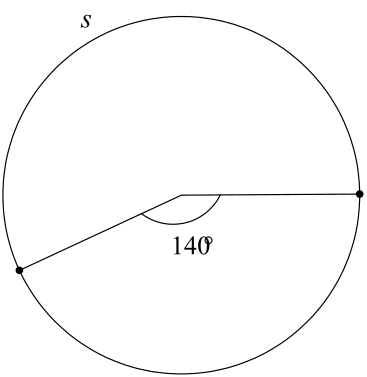
\includegraphics[ width=1.8057in, height=1.8507in,]{L4SZ281B}
}


\item [43.] Find the radius $r$ of the circle in the figure. 

\item    
\setlength\fboxrule{0in}\setlength\fboxsep{0.2in}\fcolorbox[HTML]{000000}{FFFFFF}{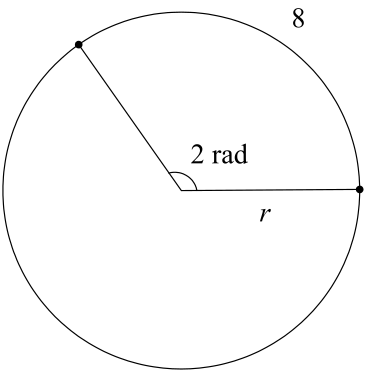
\includegraphics[ width=1.8196in, height=1.8438in,]{L4SZ281C}
}
%TCIMACRO{\TeXButton{End Two Columns}{\end {multicols}}}%
%BeginExpansion
\end {multicols}
%EndExpansion
 

\item [45.]
Find the length of an arc that subtends a central angle of $2 \mbox{rad}$ in a circle of radius 2mi. 

\item [47.]
An arc of length $100 \mbox{m}$ subtends a central angle in
a circle of radius $50 \mbox{m}$. Find the measure of $\theta $\ in degrees and in radians. 

\item [49.]
Find the radius of the circle if an arc of length $6 \mbox{m}$ on the circle subtends a central angle of $\pi /6$ rad. 

\item [51] Pittsburgh, Pennsylvania
and Miami, Florida lie approximately on the same meridian. Pittsburgh has a latitude of $40.5 \mbox{{\ensuremath{{}^\circ}}}$ N and Miami is $25.5 \mbox{{\ensuremath{{}^\circ}}}$ N. Find the distance between these two cities. (The
radius of the earth is $3960 \mbox{mi}\text{.}$) 

\item [53.] Find the distance
the earth travels in one day in its path around the sun. Assume the year has $365$ days and that the path of the earth around the sun is a circle of radius $93$ million miles. 

\item [55.] Find
the distance along an arc on the surface of the earth that subtends an angle of 1 minute. ($1$ minute = $\frac{1}{60}$ degree). This distance is called a nautical mile. The
radius of the earth is $3960 \mbox{mi}\text{.}$ 

\item [57.] Find the area
of a sector with a central angle $1 \mbox{rad}$ in a circle of radius $10 \mbox{m}$. 

\item [59.]
The area of a sector of a circle with a central angle of $2 \mbox{rad}$ is $16 \mathrm{m}^{2}$. Find the radius of the circle. 

\item [61.]
The area of the circle is $72 cm^{2}$. Find the area of a sector of the circle that subtends an angle of $\pi /6 \mbox{rad}\text{.}$ \\

\textbf{The following questions involve rotational motion and may not be covered in lecture.}

\columnsep =30pt
\begin {multicols}{2}
\item [63.]  A winch of radius $2 \mbox{ft}$ is used to lift heavy loads. If the winch makes
$8$ revolutions in $15 \mbox{s}$, find the speed at which the load is rising. 

\item
\setlength\fboxrule{0in}\setlength\fboxsep{0.2in}\fcolorbox[HTML]{000000}{FFFFFF}{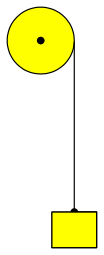
\includegraphics[ width=1.0646in, height=2.5849in,]{L4SZ281D}
}

\end {multicols}

\item [65.] A radial saw has a blade with a $6 \mbox{in}$ radius. Suppose that the blade spins at a speed
of $1000$ rpm. 

\item [(a)] Find the angular
speed of the blade in $rad/\mbox{min}\text{.}$ 

\item [(b)] Find the linear
speed of the sawteeth in $ft/\mbox{s}$. 

\item [67.] The wheels of a car have
a radius $11 \mbox{in}$ and are rotating at $600$ rpm. Find the speed of the car in $mi/\mbox{h}$. 

\item [69.] To measure the speed of
a current scientists place a paddle wheel in the stream and observe the rate at which it rotates. If the paddle
wheel has a radius $0.20 \mbox{m}$ and rotates at $100$ rpm, find the speed of the current in $\mathrm{m}/\mbox{s}$. \end{description}


%TCIMACRO{\TeXButton{Start Two Columns}{\columnsep =30pt
% \begin {multicols}{2}}}%
%BeginExpansion
\columnsep =30pt
\begin {multicols}{2}
%EndExpansion
 


%TCIMACRO{\TeXButton{End Two Columns}{\end {multicols}}}%
%BeginExpansion
\end {multicols}
%EndExpansion
 

\section{The Trigonometry of Right Triangles}


In this section we will use sine, cosine and tangent. You
should have at your fingertips the definitions of sine, cosine and tangent for a right angled triangle:
\begin{equation*}\sin  \theta  =\frac{\text{opposite}}{\text{hypotenuse}}\text{,}\cos  \theta  =\frac{\text{adjacent}}{\text{hypotenuse}}\text{and}\tan  \theta  =\frac{\text{opposite}}{\text{adjacent}}
\end{equation*}

You should be able to solve problems involving right angled triangles. A
right angled triangle is uniquely defined, if as well as the right angle, you are given two other facts about the triangle. 


\begin{enumerate}
\item Given one side and one angle 

\item Given two sides \end{enumerate}


To be given two angles does not constitute two other facts as the two angles are complementary so that given one angle the other one is known.



\begin{enumerate}
\item To solve a right triangle given one side and one angle 


\begin{description}
\item [(a)] Sketch. 

\item [(b)]
Fill in the given information and note which sides are "opp", "adj" and "hyp". 

\item [(c)]
Should the other angle be required it is found by subtraction. 

\item [(d)]
Mark the required side, pick the appropriate trigonometric ratio and solve the equation. \end{description}

\item To solve a right triangle given two sides 


\begin{description}
\item [(a)] Sketch. 

\item [(b)]
Fill in the given information. 

\item [(c)] If the third side
is required use Pythagoras theorem. 

\item [(d)] Mark the required
angle, pick the appropriate trigonometric ratio and solve the equation. (Use $\sin ^{ -1}$, $\cos ^{ -1}$ or $\tan ^{ -1}\text{.}$) \end{description}\end{enumerate}

\clearpage
\subsection{The Trigonometric Ratios of the Special Angles}
\columnsep =30pt
\begin {multicols}{2}
  
\setlength\fboxrule{0in}\setlength\fboxsep{0.2in}\fcolorbox[HTML]{000000}{FFFFFF}{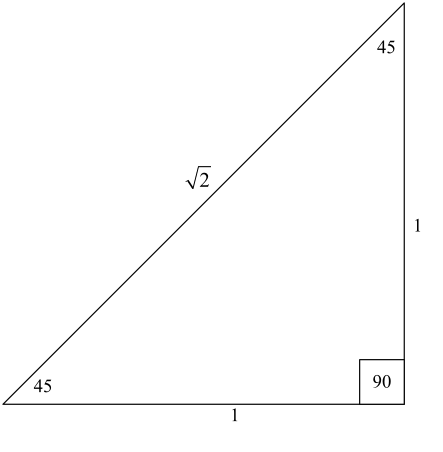
\includegraphics[ width=2.3808in, height=2.4284in,]{L4SZ281E}
}

You should be familiar with the 45, 45, 90 triangle and the ratio of the sides. Let
the two shorter sides have a length of $1$ then the hypotenuse has a length of $\sqrt{2}$. \\\relax
\begin{align*}1^{2} +1^{2} &  = 1 +1 =2 \\
\left (\sqrt{2}\right )^{2} &  = 2 \\
\text{so}1^{2} +1^{2} &  = \left (\sqrt{2}\right )^{2}\end{align*}


%TCIMACRO{\TeXButton{End Two Columns}{\end {multicols}}}%
%BeginExpansion
\end {multicols}
%EndExpansion



%TCIMACRO{\TeXButton{Start Two Columns}{\columnsep =30pt
% \begin {multicols}{2}}}%
%BeginExpansion
\columnsep =30pt
\begin {multicols}{2}
%EndExpansion
 

%   width=1.8127in, height=2.4284in,
\setlength\fboxrule{0in}\setlength\fboxsep{0.2in}\fcolorbox[HTML]{000000}{FFFFFF}{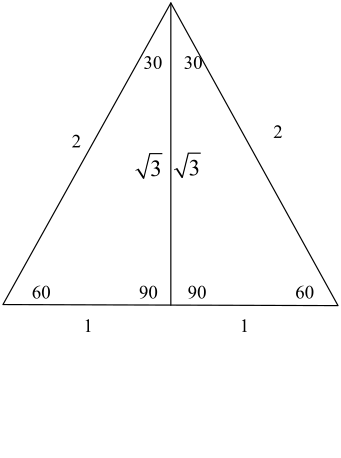
\includegraphics[ width=7cm]{L4SZ281F}
}


Similarly the equilateral triangle whose sides are 2 units gives rise to the 30, 60, 90 triangle whose sides are 1, $\sqrt{3}$ and 2. \\\relax
\begin{align*}\left (\sqrt{3}\right )^{2} +1^{2} &  =  3 +1 =4 \\
2^{2} &  =  4 \\
\text{so}\left (\sqrt{3}\right )^{2} +1^{2} &  =  2^{2}\end{align*}


\end {multicols}


The two special right triangles are the "45, 45, 90 triangle" and the "30, 60, 90 triangle". Pythagoras
theorem gives the ratio of the sides as 1, 1, $\sqrt{2}$ for the 45$\mbox{{\ensuremath{{}^\circ}}}$ 45$\mbox{{\ensuremath{{}^\circ}}}$ 90$\mbox{{\ensuremath{{}^\circ}}}$ triangle and 1, $\sqrt{3}\text{,}$ 2 for the 30$\mbox{{\ensuremath{{}^\circ}}}$ 60$\mbox{{\ensuremath{{}^\circ}}}$ 90$\mbox{{\ensuremath{{}^\circ}}}$ triangle, which is what we usually remember. 

\subsubsection{Example}
$\sin  45 \mbox{{\ensuremath{{}^\circ}}} =\frac{\text{opp}}{\text{hyp}} =\frac{1}{\sqrt{2}}$ 

We usually rationalise the denominator in expressions like $\frac{1}{\sqrt{2}}$. In other words we apply a transformation to remove the $\sqrt{2}$ from the denominator and replace it with a rational number. In this case if you multiply
the $\frac{1}{\sqrt{2}}$ by $\frac{\sqrt{2}}{\sqrt{2}}$ you get $\frac{1}{\sqrt{2}} \times \frac{\sqrt{2}}{\sqrt{2}} =\frac{\sqrt{2}}{2}$. 

Another way to achieve this is to start with the triangle 


%TCIMACRO{\TeXButton{Start Two Columns}{\columnsep =30pt
% \begin {multicols}{2}}}%
%BeginExpansion
\columnsep =30pt
\begin {multicols}{2}
%EndExpansion
 

   
\setlength\fboxrule{0in}\setlength\fboxsep{0.2in}\fcolorbox[HTML]{000000}{FFFFFF}{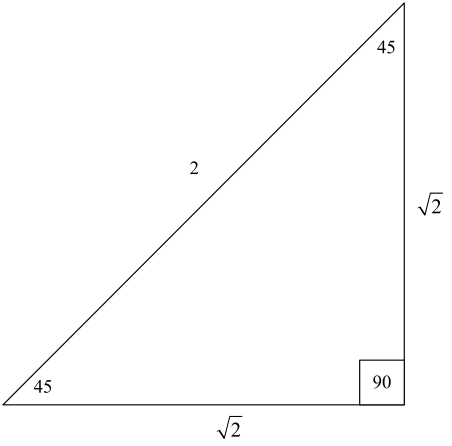
\includegraphics[ width=2.4639in, height=2.4284in,]{L4SZ281G}
}


By Pythagoras theorem
\begin{equation*}\left (\sqrt{2}\right )^{2} +\left (\sqrt{2}\right )^{2} =2 +2 =4 =2^{2}
\end{equation*}


%TCIMACRO{\TeXButton{End Two Columns}{\end {multicols}}}%
%BeginExpansion
\end {multicols}
%EndExpansion
\begin{equation*}\text{So}\sin  45 \mbox{{\ensuremath{{}^\circ}}} =\frac{\sqrt{2}}{2}\text{,}\cos  45 \mbox{{\ensuremath{{}^\circ}}} =\frac{\sqrt{2}}{2}\text{and}\tan  45 \mbox{{\ensuremath{{}^\circ}}} =\frac{\sqrt{2}}{\sqrt{2}} =1
\end{equation*}

If you are asked for the exact values of $\sin  45 \mbox{{\ensuremath{{}^\circ}}}$, $\cos  45 \mbox{{\ensuremath{{}^\circ}}}$ or $\tan  45 \mbox{{\ensuremath{{}^\circ}}}$ you should give these results. 

From the 30, 60, 90 triangle
\begin{align*}\sin  30 \mbox{{\ensuremath{{}^\circ}}} &  =  \frac{1}{2}\text{,}\cos  30 \mbox{{\ensuremath{{}^\circ}}} =\frac{\sqrt{3}}{2}\text{and}\tan  30 \mbox{{\ensuremath{{}^\circ}}} =\frac{1}{\sqrt{3}} =\frac{\sqrt{3}}{3} \\
\sin  60 \mbox{{\ensuremath{{}^\circ}}} &  = \frac{\sqrt{3}}{2}\text{,}\cos  60 \mbox{{\ensuremath{{}^\circ}}} =\frac{1}{2}\text{and}\tan  60 \mbox{{\ensuremath{{}^\circ}}} =\frac{\sqrt{3}}{1} =\sqrt{3}\end{align*}

\subsection{The Relationship between Degrees and Radians for the \\ Special Right Triangles}

\begin{align*}\sin  \frac{\pi }{4} &  =  \frac{\sqrt{2}}{2}\text{,}\cos  \frac{\pi }{4} =\frac{\sqrt{2}}{2}\text{and}\tan  \frac{\pi }{4} =\frac{\sqrt{2}}{\sqrt{2}} =1 \\
\text{So}\frac{\pi }{4} &  =  45 \mbox{{\ensuremath{{}^\circ}}}\end{align*}


\begin{align*}\sin  \frac{\pi }{6} &  =  \frac{1}{2}\text{,}\cos  \frac{\pi }{6} =\frac{\sqrt{3}}{2}\text{and}\tan  \frac{\pi }{6} =\frac{1}{\sqrt{3}} =\frac{\sqrt{3}}{3} \\
\text{So}\frac{\pi }{6} &  =  30 \mbox{{\ensuremath{{}^\circ}}}\end{align*}
\begin{align*}\sin  \frac{\pi }{3} &  =  \frac{\sqrt{3}}{2}\text{,}\cos  \frac{\pi }{3} =\frac{1}{2}\text{and}\tan  \frac{\pi }{3} =\frac{\sqrt{3}}{1} =\sqrt{3} \\
\text{So}\frac{\pi }{3} &  =  60 \mbox{{\ensuremath{{}^\circ}}}\end{align*}

The calculator gives approximate values of the trigonometric ratios. You
must look at your question to check whether angles are in degrees or radians and ensure the calculator is first set in the right \emph{mode}.
\ Remember all questions where degrees are to be used will give angles marked with a $\mbox{{\ensuremath{{}^\circ}}}$ symbol. You could assume though that when you
are dealing with a static problem (i.e. one where a triangle is given and sides and angles are required) then the angle will be measured in degrees. 

When you are required to find a side you select the trigonometric ratio and either multiply or divide.
\ When you are required to find an angle you select the appropriate trigonometry ratio and use \emph{shift}
with sin, cos or tan to find $\sin ^{ -1}$, $\cos ^{ -1}$ or $\tan ^{ -1}$ because $\sin ^{ -1}$ is said "the angle whose sine is" etc. 

\subsection{Applications}
 

\subsubsection{Example 1}
The height of a steep cliff is to be measured from a point on the opposite side of the river.  The
following diagram shows the measurements taken. Estimate the height of the cliff. 


%TCIMACRO{\TeXButton{Start Two Columns}{\columnsep =30pt
% \begin {multicols}{2}}}%
%BeginExpansion
\columnsep =30pt
\begin {multicols}{2}
%EndExpansion
 

   
\setlength\fboxrule{0in}\setlength\fboxsep{0.2in}\fcolorbox[HTML]{000000}{FFFFFF}{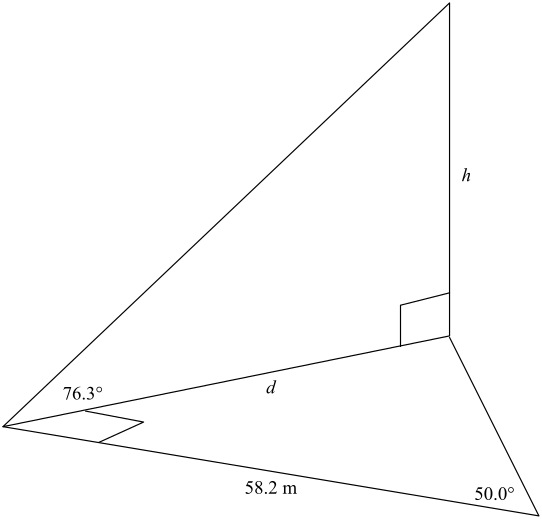
\includegraphics[ width=9cm]{L4SZ281H}
}



\begin{align*}\frac{d}{58.2} &  =  \tan  50.0 \mbox{{\ensuremath{{}^\circ}}} \\
d &  =  58.2 \times \tan  50.0 \mbox{{\ensuremath{{}^\circ}}} \\
\frac{h}{d} &  =  \tan  76.3 \mbox{{\ensuremath{{}^\circ}}} \\
h &  =  d \times \tan  76.3 \mbox{{\ensuremath{{}^\circ}}} \\
 &  =  58.2 \times \tan  50.0 \mbox{{\ensuremath{{}^\circ}}} \times \tan  76.3 \mbox{{\ensuremath{{}^\circ}}} \\
 &  \approx   284.526397 \\
 &  \approx   284.5 \mbox{m}\end{align*}


%TCIMACRO{\TeXButton{End Two Columns}{\end {multicols}}}%
%BeginExpansion
\end {multicols}
%EndExpansion


\subsubsection{Example 2}
To estimate the height of a mountain above a level plane the angle of elevation of the top of the mountain is measured to be $30 \mbox{{\ensuremath{{}^\circ}}}$. $600 \mbox{m}$ closer to the mountain across the plane it is found that the angle of elevation
is $36 \mbox{{\ensuremath{{}^\circ}}}$. Estimate the height of the mountain. 

   
\setlength\fboxrule{0in}\setlength\fboxsep{0.2in}\fcolorbox[HTML]{000000}{FFFFFF}{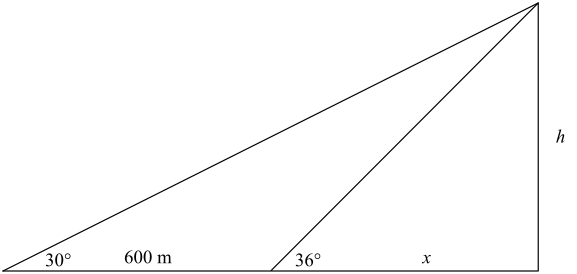
\includegraphics[ width=12cm]{L4SZ281I}
}


\begin{equation*}\frac{h}{x} =\tan  36 \mbox{{\ensuremath{{}^\circ}}}\text{and}\frac{h}{x +600} =\tan  30 \mbox{{\ensuremath{{}^\circ}}}
\end{equation*}

We want $h$ so we eliminate $x$ between these two equations
\begin{align*}x &  =  \frac{h}{\tan  36 \mbox{{\ensuremath{{}^\circ}}}}\text{and}x +600 =\frac{h}{\tan  30 \mbox{{\ensuremath{{}^\circ}}}} \\
\frac{h}{\tan  30 \mbox{{\ensuremath{{}^\circ}}}} &  =  \frac{h}{\tan  36 \mbox{{\ensuremath{{}^\circ}}}} +600 \\
\frac{h}{\tan  30 \mbox{{\ensuremath{{}^\circ}}}} -\frac{h}{\tan  36 \mbox{{\ensuremath{{}^\circ}}}} &  =  600 \\
h \left (\frac{1}{\tan  30 \mbox{{\ensuremath{{}^\circ}}}} -\frac{1}{\tan  36 \mbox{{\ensuremath{{}^\circ}}}}\right ) &  =  600 \\
h \genfrac{(}{)}{}{}{\tan  36 \mbox{{\ensuremath{{}^\circ}}} -\tan  30 \mbox{{\ensuremath{{}^\circ}}}}{\tan  30 \mbox{{\ensuremath{{}^\circ}}} \tan  36 \mbox{{\ensuremath{{}^\circ}}}} &  =  600 \\
h &  =  600 \times \frac{\tan  30 \mbox{{\ensuremath{{}^\circ}}} \tan  36 \mbox{{\ensuremath{{}^\circ}}}}{\tan  36 \mbox{{\ensuremath{{}^\circ}}} -\tan  30 \mbox{{\ensuremath{{}^\circ}}}} \\
 &  \approx   600 \times 2.811603815 \\
 &  \approx   1687 \mbox{m}\end{align*}
\clearpage
\subsubsection{Example 3}
Now use the same method to show that for 
  
\setlength\fboxrule{0in}\setlength\fboxsep{0.2in}\fcolorbox[HTML]{000000}{FFFFFF}{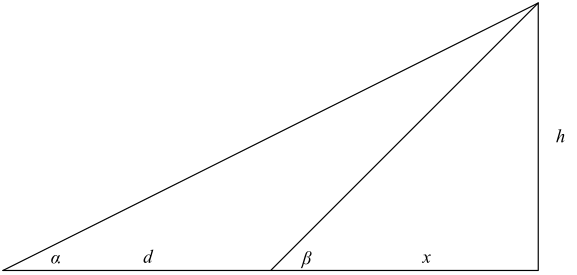
\includegraphics[ width=12cm]{L4SZ281J}
}
\begin{equation*}h =d \frac{\tan  \alpha  \tan  \beta }{\tan  \beta  -\tan  \alpha }
\end{equation*}

Let $x$ be the distance shown on the diagram.
\begin{align*}\frac{h}{x} &  =  \tan  \beta \text{and}\frac{h}{x +d} =\tan  \alpha  \\
\text{So}x &  =  \frac{h}{\tan  \beta }\text{and}x +d =\frac{h}{\tan  \alpha } \\
\text{Then}\frac{h}{\tan  \beta } +d &  =  \frac{h}{\tan  \alpha } \\
\frac{h}{\tan  \alpha } -\frac{h}{\tan  \beta } &  =  d \\
h \left (\frac{1}{\tan  \alpha } -\frac{1}{\tan  \beta }\right ) &  =  d \\
h \genfrac{(}{)}{}{}{\tan  \beta  -\tan  \alpha }{\tan  \alpha  \tan  \beta } &  =  d \\
h &  =  d \frac{\tan  \alpha  \tan  \beta }{\tan  \beta  -\tan  \alpha }\end{align*}

\subsection{Exercises}

\begin{description}
\item [1.]  Find the exact value of $\sin  \theta $, $\cos  \theta $ and $\tan  \theta $ of the angle $\theta $ in the triangle. \\
 
\columnsep =30pt
\begin {multicols}{2}  
\setlength\fboxrule{0in}\setlength\fboxsep{0.2in}\fcolorbox[HTML]{000000}{FFFFFF}{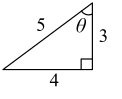
\includegraphics[ width=1.1632in, height=0.9548in,]{L4SZ281K}
}


\item [3.]  Find the angle $\theta$  
\setlength\fboxrule{0in}\setlength\fboxsep{0.2in}\fcolorbox[HTML]{000000}{FFFFFF}{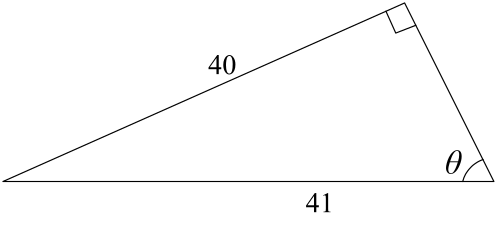
\includegraphics[ width=2.8003in, height=1.2756in,]{L4SZ281L}
}
%TCIMACRO{\TeXButton{End Two Columns}{\end {multicols}}}%
%BeginExpansion
\end {multicols}
%EndExpansion
 

\item [5.] Find the angle $\theta$
\setlength\fboxrule{0in}\setlength\fboxsep{0.2in}\fcolorbox[HTML]{000000}{FFFFFF}{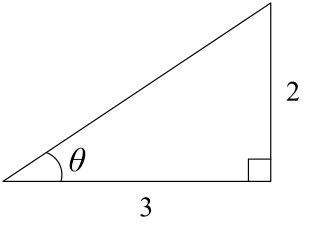
\includegraphics[ width=1.9562in, height=1.3932in,]{L4SZ281M}
}
\end{description}

Find the side labelled x. 


\begin{description}
\item [10.]   
%TCIMACRO{\TeXButton{Start Two Columns}{\columnsep =30pt
% \begin {multicols}{2}}}%
%BeginExpansion
\columnsep =30pt
\begin {multicols}{2}
%EndExpansion
    
\setlength\fboxrule{0in}\setlength\fboxsep{0.2in}\fcolorbox[HTML]{000000}{FFFFFF}{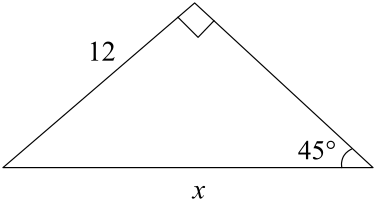
\includegraphics[ width=2.1698in, height=1.2254in,]{L4SZ281N}
}


\item [11.]    
\setlength\fboxrule{0in}\setlength\fboxsep{0.2in}\fcolorbox[HTML]{000000}{FFFFFF}{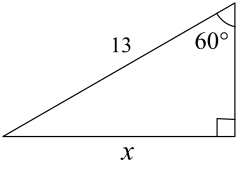
\includegraphics[ width=1.7348in, height=1.2462in,]{L4SZ281O}
}
%TCIMACRO{\TeXButton{End Two Columns}{\end {multicols}}}%
%BeginExpansion
\end {multicols}
%EndExpansion
 

\item [13.]
\setlength\fboxrule{0in}\setlength\fboxsep{0.2in}\fcolorbox[HTML]{000000}{FFFFFF}{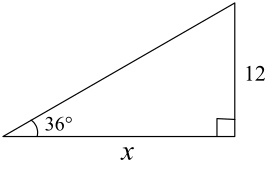
\includegraphics[ width=1.996in, height=1.2289in,]{L4SZ281P}
}
\end{description}




\begin{description}
\item [29.]   Solve the triangle 
%TCIMACRO{\TeXButton{Start Two Columns}{\columnsep =30pt
% \begin {multicols}{2}}}%
%BeginExpansion
\columnsep =30pt
\begin {multicols}{2}
%EndExpansion
    
\setlength\fboxrule{0in}\setlength\fboxsep{0.2in}\fcolorbox[HTML]{000000}{FFFFFF}{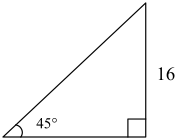
\includegraphics[ width=2.0055in, height=1.4909in,]{L4SZ281Q}
}


\item [31.]    Solve the triangle 
\setlength\fboxrule{0in}\setlength\fboxsep{0.2in}\fcolorbox[HTML]{000000}{FFFFFF}{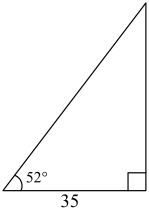
\includegraphics[ width=1.5843in, height=2.3065in,]{L4SZ281R}
}
%TCIMACRO{\TeXButton{End Two Columns}{\end {multicols}}}%
%BeginExpansion
\end {multicols}
%EndExpansion
 

\item [35.]
The angle of elevation to the top of the Empire State Building in New York is found to be $11 \mbox{{\ensuremath{{}^\circ}}}$ from the ground at a distance of $1 \mbox{mi}$ from the base of the building. Using this information,
find the height of the Empire State Building. 

\item [35.]
A laser beam is to be directed towards the centre of the moon but the beam strays $0.5 \mbox{{\ensuremath{{}^\circ}}}$ from its intended path. 

\item [(a)]
How far has the beam diverged from its assigned target when it reaches the moon? (The distance of the earth
to the moon is $240$ $000 \mbox{mi}\text{.}$) 

\item [(b)] The radius
of the moon is about $1000 \mbox{mi}$. Will the beam strike the moon? 

\item [39.]
A $20 \mbox{ft}$ ladder leans against a building so that the angle between the ground and the ladder is $72 \mbox{{\ensuremath{{}^\circ}}}$. How high does the ladder reach on the building?


\item [42.] A $96 \mbox{ft}$ tree casts a shadow that is $120 \mbox{ft}$ long. What is the angle of elevation of the sun?


\item [43.] a man is lying on the beach, flying a kite. He
holds the end of the kite string at ground level, and estimates that the angle of elevation of the kite to be $50 \mbox{{\ensuremath{{}^\circ}}}$. If the string is $450 \mbox{ft}$ long, how high is the kite above the ground? 

\item [45.]
A water tower is located $325 \mbox{ft}$ from a building. From a window in the building
it is observed that the angle of elevation to the top of the tower is $39 \mbox{{\ensuremath{{}^\circ}}}$ and the angle of depression to the bottom of the tower is $25 \mbox{{\ensuremath{{}^\circ}}}$. How tall is the tower? How
high is the window? 

\item [46.] An airplane is flying at an
elevation of $5150 \mbox{ft}$ directly above a straight highway. Two motorists
are driving cars on the highway on opposite sides of the plane and the angle of depression to one car is $35 \mbox{{\ensuremath{{}^\circ}}}$ and to the other is $52 \mbox{{\ensuremath{{}^\circ}}}$. How far apart are the cars? 

\item [49.]
To estimate the height of a mountain above a level plain, the angle of elevation to the top of the mountain is measured to be $32 \mbox{{\ensuremath{{}^\circ}}}$. One thousand feet closed to the mountain along
the plain, it is found that the angle of elevation is $35 \mbox{{\ensuremath{{}^\circ}}}$. Estimate the height of the mountain. \end{description}

 

\section{The Trigonometric Functions of Angles}


In the previous section the angles were between $0 \mbox{{\ensuremath{{}^\circ}}}$ and $90 \mbox{{\ensuremath{{}^\circ}}}$. In this section the angles can take any value.
\ Initially we consider angles between $0 \mbox{{\ensuremath{{}^\circ}}}$ and $360 \mbox{{\ensuremath{{}^\circ}}}$ and relate these to the radian measure between $0$ and $2 \pi $. We remind you that angles are measured anticlockwise from the positive $x$-axis. 

If the point $P (x ,y)$ is in the first quadrant, $\theta $ is the angle between $OP$ and the positive $x$-axis and we complete the right triangle then we have created the following situation.  
%TCIMACRO{\TeXButton{Start Two Columns}{\columnsep =30pt
% \begin {multicols}{2}}}%
%BeginExpansion
\columnsep =30pt
\begin {multicols}{2}
%EndExpansion
 

   
\setlength\fboxrule{0in}\setlength\fboxsep{0.2in}\fcolorbox[HTML]{000000}{FFFFFF}{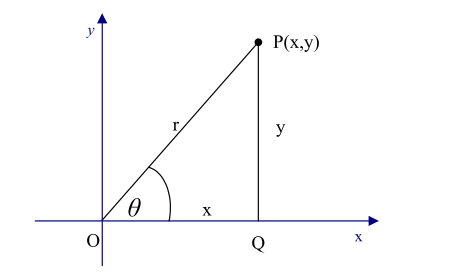
\includegraphics[ width=3.774in, height=2.3454in,]{L4SZ281S}
}


Let the hypotenuse be $r$ then
\begin{equation*}r =\sqrt{x^{2} +y^{2}}
\end{equation*}


%TCIMACRO{\TeXButton{End Two Columns}{\end {multicols}}}%
%BeginExpansion
\end {multicols}
%EndExpansion


Therefore
\begin{equation*}\sin  \theta  =\frac{y}{r}\text{}\cos  \theta  =\frac{x}{r}\text{and}\tan  \theta  =\frac{y}{x}
\end{equation*}

We now let $\theta $ be any angle and define sine, cosine and tangent in the same way. For instance
if $P (x ,y)$ is in the second quadrant: 

   
\setlength\fboxrule{0in}\setlength\fboxsep{0.2in}\fcolorbox[HTML]{000000}{FFFFFF}{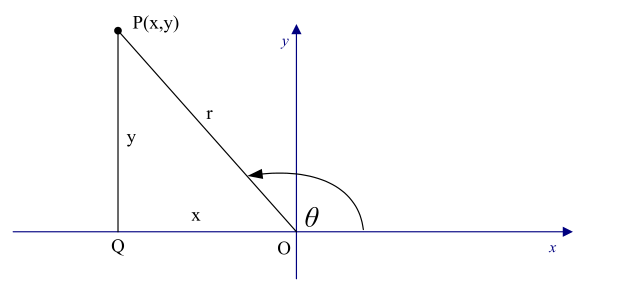
\includegraphics[ width=3.9868in, height=1.8161in,]{L4SZ281T}
}


$\sin  \theta  =\frac{y}{r}$ because $y$ is positive $\sin  \theta $ will be positive. ($r$ is positive by convention.) 

$\cos  \theta  =\frac{x}{r}$ because $x$ is negative $\cos  \theta $ will be negative. 

$\tan  \theta  =\frac{y}{x}$ because $y$ is positive and $x$ is negative $\tan  \theta $ will be negative. 

This pattern can be extended to quadrants 3 and 4. The
mnemonic (\textbf{A}ll \textbf{S}tudents \textbf{T}ake \textbf{C}alculus) might help you remember which one is positive
although you can always work it out if you need to. 

%\subsection{Relating Angles between 0$\mbox{{\ensuremath{{}^\circ}}}$ and 360$\mbox{{\ensuremath{{}^\circ}}}$ to an Equivalent Angle between 0$\mbox{{\ensuremath{{}^\circ}}}$ and 90$\mbox{{\ensuremath{{}^\circ}}}$}
%By constructing $\bar{PQ}$ perpendicular to the $x$-axis a triangle is formed and this can be transformed into a congruent triangle in the first quadrant.This
%is particularly important if an exact value is required for one of the special angles. 
%
%\subsubsection{Example 1}
%Given $\sin  60 \mbox{{\ensuremath{{}^\circ}}} =\frac{\sqrt{3}}{2}$ it can be shown $\sin  120 \mbox{{\ensuremath{{}^\circ}}} =\frac{\sqrt{3}}{2}$, $\sin  240 \mbox{{\ensuremath{{}^\circ}}} = -\frac{\sqrt{3}}{2}$ and $\sin  300 \mbox{{\ensuremath{{}^\circ}}} = -\frac{\sqrt{3}}{2}$ 
%
%\subsubsection{Example 2}
%Given $\cos  45 \mbox{{\ensuremath{{}^\circ}}} =\frac{\sqrt{2}}{2}$ it can be shown $\cos  135 \mbox{{\ensuremath{{}^\circ}}} = -\frac{\sqrt{2}}{2}$, $\cos  225 \mbox{{\ensuremath{{}^\circ}}} = -\frac{\sqrt{2}}{2}$ and $\cos  315 \mbox{{\ensuremath{{}^\circ}}} =\frac{\sqrt{2}}{2}$ 
%
%This can be continued beyond $360 \mbox{{\ensuremath{{}^\circ}}}$. 
%
%\subsubsection{Example 3}
%Given $\tan  30 \mbox{{\ensuremath{{}^\circ}}} =\frac{\sqrt{3}}{3}$ it can be shown $\tan  390 \mbox{{\ensuremath{{}^\circ}}} =\frac{\sqrt{3}}{3}$, $\tan  510 \mbox{{\ensuremath{{}^\circ}}} = -\frac{\sqrt{3}}{3}$, $\tan  570 \mbox{{\ensuremath{{}^\circ}}} =\frac{\sqrt{3}}{3}$ and $\tan  690 \mbox{{\ensuremath{{}^\circ}}} = -\frac{\sqrt{3}}{3}$ 
%
%This also holds for angles measured in a clockwise direction 
%
%\subsubsection{Example 4}
%Given $\tan  45 \mbox{{\ensuremath{{}^\circ}}} =1$ it can be shown $\tan  -45 \mbox{{\ensuremath{{}^\circ}}} = -1$, $\tan  -135 \mbox{{\ensuremath{{}^\circ}}} = -1$, $\tan  -225 \mbox{{\ensuremath{{}^\circ}}} = -1$ and $\tan  -315 \mbox{{\ensuremath{{}^\circ}}} =1$ 
%
%The textbook refers to this as finding the \emph{reference angle}. We
%will avoid this additional definition, however the procedure of finding the congruent triangle in the first quadrant must be understood. Although
%the same logic can be applied to \emph{any} angle in that a congruent triangle can be constructed in the first quadrant we will only bother
%to do this for the special angles. For all other angles the calculator gives an approximate value. You
%should note therefore whether a special angle is given where an exact answer is expected or whether an approximate answer will suffice. 

\subsection{The Area of a Triangle}
The fundamental formula for the area of a triangle is
\begin{equation*}\text{Area} =\frac{1}{2} \times \text{base} \times \text{height}
\end{equation*}

Using the trigonometric functions the height can be replaced
and the formula becomes
\begin{equation*}\text{Area} =\frac{1}{2} \times \text{product of two sides} \times \text{sine of the included angle}
\end{equation*}

The formula is particularly easy to remember in symbolic form. Let
the triangle have vertices $A$, $B$ and $C$, so the the sides opposite these angles are $a$, $b$ and $c$ respectively. Then the area can be expressed symbolically as
\begin{equation*}\text{Area} =\frac{1}{2} a b \sin  C =\frac{1}{2} b c \sin  A =\frac{1}{2} a c \sin  B
\end{equation*}


%TCIMACRO{\TeXButton{Start Two Columns}{\columnsep =30pt
% \begin {multicols}{2}}}%
%BeginExpansion
\columnsep =30pt
\begin {multicols}{2}
%EndExpansion
 

   
\setlength\fboxrule{0in}\setlength\fboxsep{0.2in}\fcolorbox[HTML]{000000}{FFFFFF}{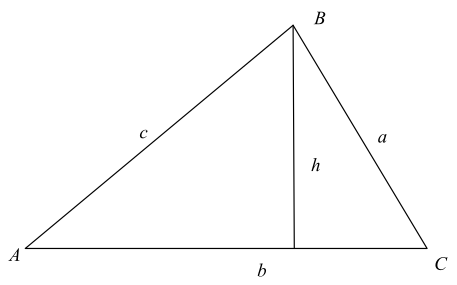
\includegraphics[ width=3.1012in, height=1.9415in,]{L4SZ281U}
}



\begin{align*}\sin  A &  = \frac{h}{c}\text{so}h =c \sin  A \\
\text{Area} &  =  \frac{1}{2} \times \text{base} \times \text{height} \\
 &  =  \frac{1}{2} \times b \times c \sin  A =\frac{1}{2} b c \sin  A\end{align*}


%TCIMACRO{\TeXButton{End Two Columns}{\end {multicols}}}%
%BeginExpansion
\end {multicols}
%EndExpansion


It depends where you draw $h$ and which angle you choose to use as to which formula you finish up with. The key
point to remember is $b$ and $c$ are two sides and $A$ is the angle between them. The triangle above shows $A$ as an acute angle (between $0$ and $90 \mbox{{\ensuremath{{}^\circ}}}$). If the angle is obtuse (between $90 \mbox{{\ensuremath{{}^\circ}}}$ and $180 \mbox{{\ensuremath{{}^\circ}}}$) the formula still holds. 

   
\setlength\fboxrule{0in}\setlength\fboxsep{0.2in}\fcolorbox[HTML]{000000}{FFFFFF}{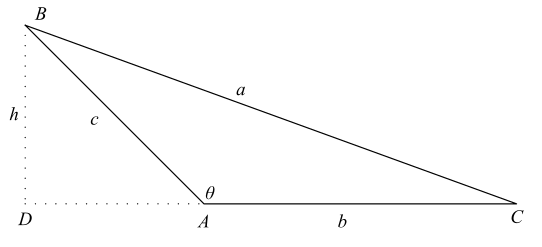
\includegraphics[ width=3.6573in, height=1.6769in,]{L4SZ281V}
}


The angle is in the second quadrant and $\sin  (180 -\theta ) =\sin  \theta $, so $\sin  (180 -\theta ) =\frac{h}{c}$ can be written as $\sin  \theta  =\frac{h}{c}$ or $h =c \sin  \theta $ or $h =c \sin  A$ where $A$ is obtuse. So the area is $\frac{1}{2} b c \sin  A$ 

\subsubsection{Example 5}
A triangle has two sides of $5 \mbox{cm}$ and $8 \mbox{cm}$ and the angle between them is $150 \mbox{{\ensuremath{{}^\circ}}}$. Find its area.
\begin{equation*}\text{Area} =\frac{1}{2} \times 5 \times 8 \times \sin  150 \mbox{{\ensuremath{{}^\circ}}}
\end{equation*}

It helps to remember that $\sin  150 =\sin  30 =\frac{1}{2}$
\begin{equation*}\text{Area} =\frac{1}{2} \times 5 \times 8 \times \frac{1}{2} =10 cm^{2}
\end{equation*}

\subsection{Exercises}
Find the exact value of the trigonometric function
\begin{description}
\item [7.]   
%TCIMACRO{\TeXButton{Start Two Columns}{\columnsep =30pt
% \begin {multicols}{2}}}%
%BeginExpansion
\columnsep =30pt
\begin {multicols}{2}
%EndExpansion
 $\sin  150 \mbox{{\ensuremath{{}^\circ}}}$ 

\item [9.] $\cos  135 \mbox{{\ensuremath{{}^\circ}}}$ 
%TCIMACRO{\TeXButton{End Two Columns}{\end {multicols}}}%
%BeginExpansion
\end {multicols}
%EndExpansion
 

\item [11.]
%TCIMACRO{\TeXButton{Start Two Columns}{\columnsep =30pt
% \begin {multicols}{2}}}%
%BeginExpansion
\columnsep =30pt
\begin {multicols}{2}
%EndExpansion
 $\tan  \left ( -60 \mbox{{\ensuremath{{}^\circ}}}\right )$ 

\item [15.] $\cos  570 \mbox{{\ensuremath{{}^\circ}}}$ 
%TCIMACRO{\TeXButton{End Two Columns}{\end {multicols}}}%
%BeginExpansion
\end {multicols}
%EndExpansion
  

\item [17.]   
%TCIMACRO{\TeXButton{Start Two Columns}{\columnsep =30pt
% \begin {multicols}{2}}}%
%BeginExpansion
\columnsep =30pt
\begin {multicols}{2}
%EndExpansion
 $\tan  750 \mbox{{\ensuremath{{}^\circ}}}$ 

\item [19.] $\sin  \frac{2 \pi }{3}$ 
%TCIMACRO{\TeXButton{End Two Columns}{\end {multicols}}}%
%BeginExpansion
\end {multicols}
%EndExpansion
 

\item [21.]
%TCIMACRO{\TeXButton{Start Two Columns}{\columnsep =30pt
% \begin {multicols}{2}}}%
%BeginExpansion
\columnsep =30pt
\begin {multicols}{2}
%EndExpansion
 $\sin  \frac{3 \pi }{2}$ 

\item [23.] $\cos  \left ( -\frac{7 \pi }{3}\right )$ 
%TCIMACRO{\TeXButton{End Two Columns}{\end {multicols}}}%
%BeginExpansion
\end {multicols}
%EndExpansion
 

\item [29.]
$\tan  \frac{5 \pi }{2}$ \end{description}

Find the value of the trigonometric functions of $\theta $ from the information given 


\begin{description}
\item [41.] $\sin  \theta  =\frac{3}{5}\text{,}$ $\theta $ in quadrant II 

\item [43.]
$\tan  \theta  = -\frac{3}{4}\text{,}$ $\cos  \theta  >0$ 

\item [49.] If $\theta  =\pi /3\text{,}$ find the value of each expression. 

\item [(a)]
%TCIMACRO{\TeXButton{Start Two Columns}{\columnsep =30pt
% \begin {multicols}{2}}}%
%BeginExpansion
\columnsep =30pt
\begin {multicols}{2}
%EndExpansion
 $\sin  2 \theta \text{,}$ $2 \sin  \theta $ 

\item [(b)] $\sin  \frac{1}{2} \theta \text{,}$ $\frac{\sin  \theta }{2}$ 
%TCIMACRO{\TeXButton{End Two Columns}{\end {multicols}}}%
%BeginExpansion
\end {multicols}
%EndExpansion
 

\item [(c)]
$\sin ^{2} \theta \text{,}$ $\sin  \left (\theta ^{2}\right )$ 

\item [51.] Find the area of a triangle
with sides of length $7$ and $9$ and included angle $72 \mbox{{\ensuremath{{}^\circ}}}$. 

\item [53.]
A triangle has an area of $16 in^{2}\text{,}$ and two of the sides of the triangle have lengths $5 \mbox{in}$ and $7 \mbox{in}$. Find the angle included by these two sides. \end{description}


%TCIMACRO{\TeXButton{Start Two Columns}{\columnsep =30pt
% \begin {multicols}{2}}}%
%BeginExpansion
\columnsep =30pt
\begin {multicols}{2}
%EndExpansion
 


%TCIMACRO{\TeXButton{End Two Columns}{\end {multicols}}}%
%BeginExpansion
\end {multicols}
%EndExpansion
 

\section{The Sine Rule}


In this section we use the Sine Rule to find the sides and angles in triangles without a right angle.
\ In the next section we use the Cosine Rule to find sides and angles in triangles also, so as you study these
two sections you need to learn which problems require the Sine Rule and which require the Cosine Rule. 

Previously, we met the formula
for the area of a triangle. given two sides and the included angle $\left ( =\frac{1}{2} a b \sin  C\right )$. The Sine Rule and
Cosine Rule also require specific combinations of sides and angles. 

The easiest way to visualise the situations in which the two rules
are used is to use the labelling we met in section $3.3$. Let the triangle be $ \Delta A B C$ and let the sides be $a$, $b$ and $c$ where $a$ is opposite $\angle A$ etc. 

   
\setlength\fboxrule{0in}\setlength\fboxsep{0.2in}\fcolorbox[HTML]{000000}{FFFFFF}{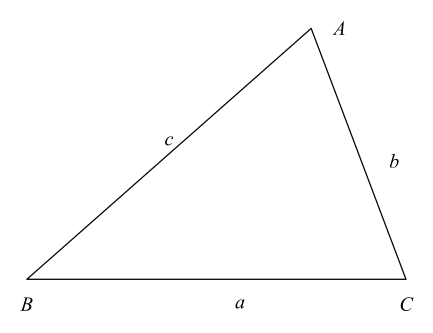
\includegraphics[ width=3.1358in, height=2.4171in,]{L4SZ281W}
}



\begin{tabular}[c]{lll}\textbf{Sine Rule}  &  & \textbf{Cosine
Rule}  \\
 Given a side and the angle opposite the side  &  & \textbf{(a)}
Given two sides and the included angle  \\
 \textbf{(a)} If a second angle is
given the Sine Rule  &  & the Cosine Rule allows us to find the
side  \\
allows us the side opposite that angle  &  & opposite
the angle  \\
Given $A$, $a$ and $B$ use the Sine Rule to find $b\text{.}$  &  & Given $a$, $b$ and $C$ use the Cosine Rule to find $c\text{.}$  \\
 \textbf{(b)} If a second
angle is given and the side that  &  & \textbf{(b)} Given three
sides the Cosine Rule allows  \\
is not opposite that angle is required then first  &  & us
to find any angle.  \\
find the third angle then use (a).  &  & Given
$a$, $b$ and $c$ use the Cosine Rule to find $A$  \\
Given $A$, $a$ and $B$ where $c$ is required  &  & or $B$ or $C$.  \\
 1. $C =180 -(A +B)$  &  &  \\
2.
Use the Sine Rule to find $c$.  &  &  \\
\textbf{(c)} If a second side is given the Sine Rule  &  &  \\
allows
us to find the angle opposite that side.  &  &  \\
Given
$A$, $a$, and $b$ use the Sine Rule to find $B$.  &  &  \\
\end{tabular}

Textbooks may use the term ``The Law of Sines" whereas in these notes the term
``The Sine Rule will be used. 

The Sine Rule states that in any triangle
\begin{equation*}\frac{\sin  A}{a} =\frac{\sin  B}{b} =\frac{\sin  C}{c}
\end{equation*}

or
\begin{equation*}\frac{a}{\sin  A} =\frac{b}{\sin  B} =\frac{c}{\sin  C}
\end{equation*}

\subsection{Proof of the Sine Rule}
The Sine Rule is easy to prove from the formula for the area of a triangle
\begin{equation*}\text{Area} =\frac{1}{2} b c \sin  A =\frac{1}{2} a c \sin  B =\frac{1}{2} a b \sin  C
\end{equation*}

Multiply right through by 2
\begin{equation*}b c \sin  A =a c \sin  B =a b \sin  C
\end{equation*}

Divide right through by $a b c$
\begin{equation*}\frac{\sin  A}{a} =\frac{\sin  B}{b} =\frac{\sin  C}{c}
\end{equation*}

Fractions can always be inverted as long as the same process is applied to each fraction.
\begin{equation*}\frac{a}{\sin  A} =\frac{b}{\sin  B} =\frac{c}{\sin  C}
\end{equation*}

\subsubsection{Example 1}
   
\setlength\fboxrule{0in}\setlength\fboxsep{0.2in}\fcolorbox[HTML]{000000}{FFFFFF}{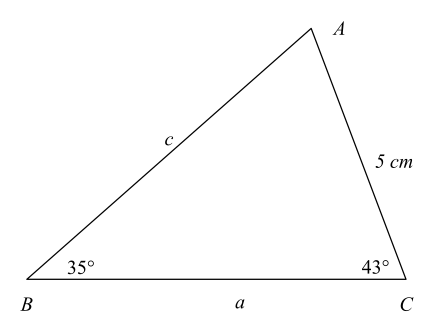
\includegraphics[ width=2.6143in, height=2.0159in,]{L4SZ281X}
}
\\\relax (a) To find $c$
\begin{align*}\frac{c}{\sin  C} &  = \frac{b}{\sin  B} \\
\frac{c}{\sin  43 \mbox{{\ensuremath{{}^\circ}}}} &  = \frac{5}{\sin  35 \mbox{{\ensuremath{{}^\circ}}}} \\
c &  = \frac{5 \sin  43 \mbox{{\ensuremath{{}^\circ}}}}{\sin  35 \mbox{{\ensuremath{{}^\circ}}}} \\
 &  \approx   5.945139277 \approx 5.9 \mbox{cm}\text{(1 dp)}\end{align*} \\\relax (b) To find $a$ 

(i) $A =180 \mbox{{\ensuremath{{}^\circ}}} -(35 \mbox{{\ensuremath{{}^\circ}}} +43 \mbox{{\ensuremath{{}^\circ}}}) =180 \mbox{{\ensuremath{{}^\circ}}} -78 \mbox{{\ensuremath{{}^\circ}}} =102 \mbox{{\ensuremath{{}^\circ}}}$ 

(ii) It is usually wise to go back to the original data (i.e. use $b$ and $B$ rather than $c$ and $C$).
\begin{align*}\frac{a}{\sin  A} &  = \frac{b}{\sin  B} \\
\frac{a}{\sin  102 \mbox{{\ensuremath{{}^\circ}}}} &  = \frac{5}{\sin  35 \mbox{{\ensuremath{{}^\circ}}}} \\
a &  = \frac{5 \sin  102 \mbox{{\ensuremath{{}^\circ}}}}{\sin  35 \mbox{{\ensuremath{{}^\circ}}}} \\
 &  \approx   8.526741501 \approx 8.5 \mbox{cm}\text{(1 dp)}\end{align*}

These two calculations
illustrate the first two cases in which the Sine Rule is used. You will notice that the triangle has been completely
solved in the course of this example. We started with one side and two angles and we found the other two sides
and the other angle. 

The third case is not as straight forward. Given two sides and an
angle there could be no triangle formed, one triangle formed or two triangles formed depending on the length of the side opposite the given angle. You should develop an insight into the reasons why
this is so. Imagine the second side given is the boom of a crane and the angle given is the angle between the
boom and the ground. The side opposite the given angle is represented by the cable. It is clear that for certain
lengths of the cable the hook will not reach the ground. Then as the hook is lowered a point will be reached
when the hook just touches the ground.  
%TCIMACRO{\TeXButton{Start Two Columns}{\columnsep =30pt
% \begin {multicols}{2}}}%
%BeginExpansion
\columnsep =30pt
\begin {multicols}{2}
%EndExpansion
 

   
\setlength\fboxrule{0in}\setlength\fboxsep{0.2in}\fcolorbox[HTML]{000000}{FFFFFF}{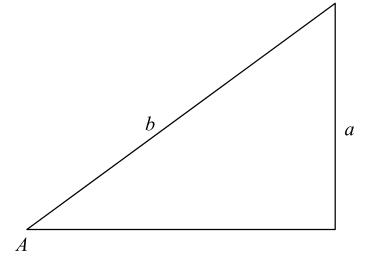
\includegraphics[ width=2.9577in, height=2.2061in,]{L4SZ281Y}
}


It is no surprise that the length $a$ to create this situation is $a =b \sin  A\text{.}$ 

We are after all dealing with the Sine Rule which becomes the fundamental sine formula $\left (\sin  A =\frac{\text{opp}}{\text{hyp}} =\frac{a}{b}\right )$ when the triangle has a right angle. 
%TCIMACRO{\TeXButton{End Two Columns}{\end {multicols}}}%
%BeginExpansion
\end {multicols}
%EndExpansion


If the cable is held taut and is extended a little more it will touch the ground in two places (provided it is kept in the same plane).
\ As the cable is extended further the time will come where the cable is as long as boom. At
this point there is only one solution again, the one straight out in front of the crane). Further extensions
of the cable will produce only one solution (straight out in front of the crane) as the cable will theoretically reach behind the crane boom thus creating
a different triangle altogether. 

The two solutions case is often referred to as the ambiguous case. The
discussion above shows the range of values of $a$ that will give two solutions.
\begin{equation*}b \sin  A <a <b
\end{equation*}

\subsubsection{Example 2}
Given $a =30 \mbox{{\ensuremath{{}^\circ}}}$, $a =8$ and $b =7$ solve the triangle (i.e. find $B$, $C$ and $c$). 

   
\setlength\fboxrule{0in}\setlength\fboxsep{0.2in}\fcolorbox[HTML]{000000}{FFFFFF}{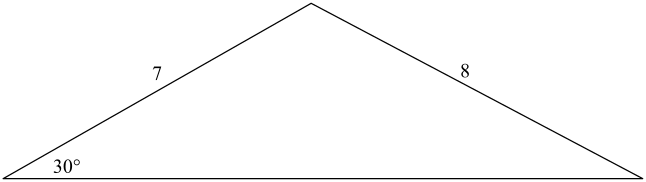
\includegraphics[ width=4.2739in, height=1.2202in,]{L4SZ281Z}
}


Because $8 >7$ this is the one solution case. 

1. Find $B$
\begin{align*}\frac{\sin  B}{b} &  = \frac{\sin  A}{a} \\
\sin  B &  = \frac{b \sin  A}{a} \\
 &  = \frac{7 \sin  30 \mbox{{\ensuremath{{}^\circ}}}}{8} =0.4375 \\
B &  = \sin ^{ -1} 0.4375 \approx 25.94 \mbox{{\ensuremath{{}^\circ}}}\end{align*}

2. Find $C$
\begin{align*}C &  = 180 \mbox{{\ensuremath{{}^\circ}}} -(30 \mbox{{\ensuremath{{}^\circ}}} +25.94 \mbox{{\ensuremath{{}^\circ}}}) \\
 &  = 124.06 \mbox{{\ensuremath{{}^\circ}}}\end{align*}

3. Find $c$
\begin{align*}\frac{c}{\sin  C} &  = \frac{a}{\sin  A} \\
c &  = \frac{a \sin  C}{c} \\
 &  = \frac{7 \sin  124.06 \mbox{{\ensuremath{{}^\circ}}}}{\sin  30 \mbox{{\ensuremath{{}^\circ}}}} \\
 &  \approx   11.6\end{align*}

\subsubsection{Example 3}
Given $A =30 \mbox{{\ensuremath{{}^\circ}}}$, $a =6$ and $b =7$ solve the triangle. 

In this case $b \sin  A =3.5$ and $b =7$ so as $a$ lies between $3.5$ and $7$. This is the ambiguous case, therefore there are two solutions. 


%TCIMACRO{\TeXButton{Start Two Columns}{\columnsep =30pt
% \begin {multicols}{2}}}%
%BeginExpansion
\columnsep =30pt
\begin {multicols}{2}
%EndExpansion
 

   
\setlength\fboxrule{0in}\setlength\fboxsep{0.2in}\fcolorbox[HTML]{000000}{FFFFFF}{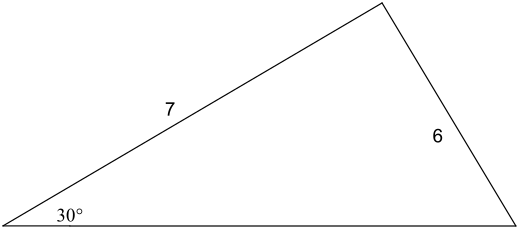
\includegraphics[ width=2.8885in, height=1.2825in,]{L4SZ2820}
}


   
\setlength\fboxrule{0in}\setlength\fboxsep{0.2in}\fcolorbox[HTML]{000000}{FFFFFF}{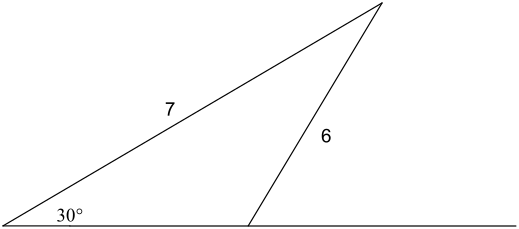
\includegraphics[ width=2.9308in, height=1.3015in,]{L4SZ2821}
}



%TCIMACRO{\TeXButton{End Two Columns}{\end {multicols}}}%
%BeginExpansion
\end {multicols}
%EndExpansion
 

It
is best to visualise these two solutions on the same diagram so that the isosceles triangle can help lead to the two results. 

   
\setlength\fboxrule{0in}\setlength\fboxsep{0.2in}\fcolorbox[HTML]{000000}{FFFFFF}{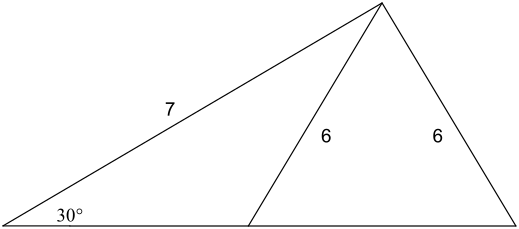
\includegraphics[ width=2.9585in, height=1.3136in,]{L4SZ2822}
}


 \textbf{First solution} (Proceed as before) 

1. Find $B$
\begin{align*}\frac{\sin  B}{b} &  = \frac{\sin  A}{a} \\
\sin  B &  = \frac{b \sin  A}{a} \\
 &  = \frac{7 \sin  30 \mbox{{\ensuremath{{}^\circ}}}}{6} =0.58 \dot{3} \\
B &  = \sin ^{ -1} 0.58 \dot{3} \approx 35.69 \mbox{{\ensuremath{{}^\circ}}}\end{align*}

2. Find $C$
\begin{align*}C &  = 180 \mbox{{\ensuremath{{}^\circ}}} -(30 \mbox{{\ensuremath{{}^\circ}}} +35.69 \mbox{{\ensuremath{{}^\circ}}}) \\
 &  = 114.31 \mbox{{\ensuremath{{}^\circ}}}\end{align*}

3. Find $c$
\begin{align*}\frac{c}{\sin  C} &  = \frac{a}{\sin  A} \\
c &  = \frac{a \sin  C}{\sin  A} \\
 &  = \frac{6 \sin  114.31 \mbox{{\ensuremath{{}^\circ}}}}{\sin  30 \mbox{{\ensuremath{{}^\circ}}}} \\
 &  \approx   10.9\end{align*}

\textbf{Second solution} 

1. Find the second value of $B$ 

\begin{equation*}B =180 \mbox{{\ensuremath{{}^\circ}}} -35.69 \mbox{{\ensuremath{{}^\circ}}} =144.31 \mbox{{\ensuremath{{}^\circ}}}
\end{equation*}

2. Find $C$
\begin{equation*}C =180 \mbox{{\ensuremath{{}^\circ}}} -(30 \mbox{{\ensuremath{{}^\circ}}} +144.31 \mbox{{\ensuremath{{}^\circ}}}) =180 \mbox{{\ensuremath{{}^\circ}}} -174.31 \mbox{{\ensuremath{{}^\circ}}} =5.69 \mbox{{\ensuremath{{}^\circ}}}
\end{equation*}

(Or if you remember the rule that the exterior angle of a triangle is the sum of the two interior
opposite angles $C +30 \mbox{{\ensuremath{{}^\circ}}} =35.69 \mbox{{\ensuremath{{}^\circ}}}$ so $C =35.69 \mbox{{\ensuremath{{}^\circ}}} -30 \mbox{{\ensuremath{{}^\circ}}} =5.69 \mbox{{\ensuremath{{}^\circ}}}$) 

3. Find $c$
\begin{align*}\frac{c}{\sin  C} &  = \frac{a}{\sin  A} \\
c &  = \frac{a \sin  C}{\sin  A} \\
 &  = \frac{6 \sin  5.69 \mbox{{\ensuremath{{}^\circ}}}}{\sin  30 \mbox{{\ensuremath{{}^\circ}}}} \\
 &  \approx   1.2\end{align*}

%\subsection{ }


\subsection{Exercises}

Use the Sine Rule to find side $x$ or angle $\theta $  
%TCIMACRO{\TeXButton{Start Two Columns}{\columnsep =30pt
% \begin {multicols}{2}}}%
%BeginExpansion
\columnsep =30pt
\begin {multicols}{2}
%EndExpansion
 


%TCIMACRO{\TeXButton{End Two Columns}{\end {multicols}}}%
%BeginExpansion
\end {multicols}
%EndExpansion



\begin{description}
\item [1.]   
%TCIMACRO{\TeXButton{Start Two Columns}{\columnsep =30pt
% \begin {multicols}{2}}}%
%BeginExpansion
\columnsep =30pt
\begin {multicols}{2}
%EndExpansion
    
\setlength\fboxrule{0in}\setlength\fboxsep{0.2in}\fcolorbox[HTML]{000000}{FFFFFF}{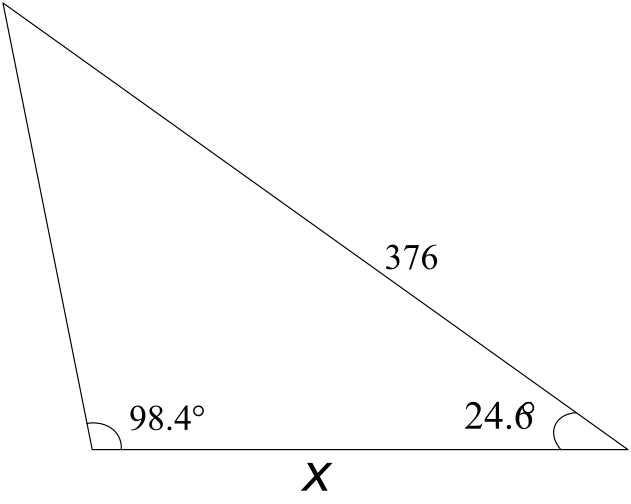
\includegraphics[ width=2.2373in, height=1.7902in,]{L4SZ2823}
}


\item [5]    
\setlength\fboxrule{0in}\setlength\fboxsep{0.2in}\fcolorbox[HTML]{000000}{FFFFFF}{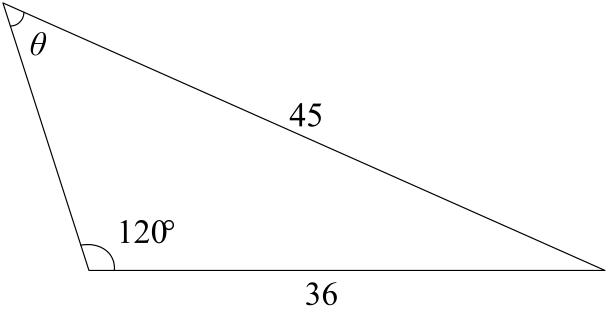
\includegraphics[ width=2.3609in, height=1.241in,]{L4SZ2824}
}
%TCIMACRO{\TeXButton{End Two Columns}{\end {multicols}}}%
%BeginExpansion
\end {multicols}
%EndExpansion
 \end{description}

Solve the triangle using the Sine Rule. 


\begin{description}
\item [7.]    
\setlength\fboxrule{0in}\setlength\fboxsep{0.2in}\fcolorbox[HTML]{000000}{FFFFFF}{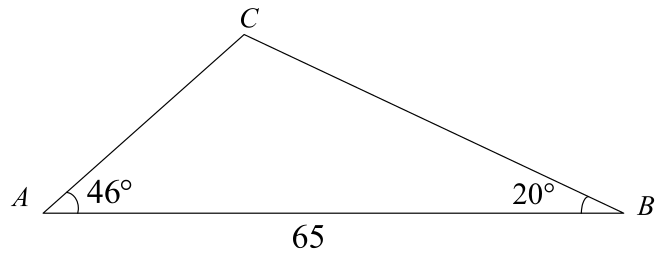
\includegraphics[ width=3.5198in, height=1.3863in,]{L4SZ2825}
}
\end{description}

Sketch each triangle and then solve the triangle using the Sine Rule. 


\begin{description}
\item [9.] $\angle A =50 \mbox{{\ensuremath{{}^\circ}}}\text{,}$ $\angle B =68 \mbox{{\ensuremath{{}^\circ}}}\text{,}$ $c =230$ 

\item [13.] $\angle B =29 \mbox{{\ensuremath{{}^\circ}}}\text{,}$ $\angle C =51 \mbox{{\ensuremath{{}^\circ}}}\text{,}$ $b =44$ 

\item [23.]   
%TCIMACRO{\TeXButton{Start Two Columns}{\columnsep =30pt
% \begin {multicols}{2}}}%
%BeginExpansion
\columnsep =30pt
\begin {multicols}{2}
%EndExpansion
 To find the distance across a river, a surveyor chooses points $A$ and $B$, which are $200 \mbox{ft}$ apart on one side of the river. She then chooses
a reference point $C$ on the opposite side of the river and finds that $\angle BAC \approx 82 \mbox{{\ensuremath{{}^\circ}}}$ and $\angle ABC \approx 52 \mbox{{\ensuremath{{}^\circ}}}\text{.}$  Find the approximate
distance from $A$ to $C$. 

\item    
\setlength\fboxrule{0in}\setlength\fboxsep{0.2in}\fcolorbox[HTML]{000000}{FFFFFF}{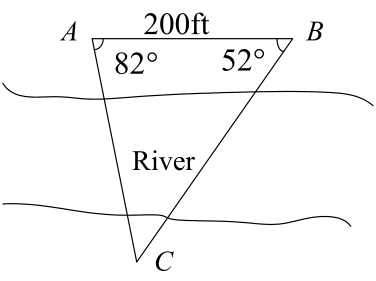
\includegraphics[ width=2.4059in, height=1.7988in,]{L4SZ2826}
}
%TCIMACRO{\TeXButton{End Two Columns}{\end {multicols}}}%
%BeginExpansion
\end {multicols}
%EndExpansion
 

\item [25.]
The path of a satellite circling the earth causes it to pass directly over two tracking stations $A$ and $B$, which are $50 \mbox{mi}$ apart. When the satellite is on one side of the
two stations, the angle of elevation at $A$ and $B$ are measured to be $87.0 \mbox{{\ensuremath{{}^\circ}}}$ and $84.2 \mbox{{\ensuremath{{}^\circ}}}$, respectively. 

\item [(a)]
Draw a diagram. 

\item [(b)] How far is the satellite from
station $A$? 

\item [(c)] How high is the satellite
above the ground? 

\item [27.]   
%TCIMACRO{\TeXButton{Start Two Columns}{\columnsep =30pt
% \begin {multicols}{2}}}%
%BeginExpansion
\columnsep =30pt
\begin {multicols}{2}
%EndExpansion
 A communication tower is located at the top of a steep hill. The angle of inclination
of the hill is $58 \mbox{{\ensuremath{{}^\circ}}}$. A guy wire is attached to the top of the tower
and to the ground, $100 \mbox{m}$ downhill from the base of the tower. The
angle between the slope of the hill and the guy wire is measured as $12 \mbox{{\ensuremath{{}^\circ}}}$. Find $A C$, the length of cable required for the guy wire. 

\item    
\setlength\fboxrule{0in}\setlength\fboxsep{0.2in}\fcolorbox[HTML]{000000}{FFFFFF}{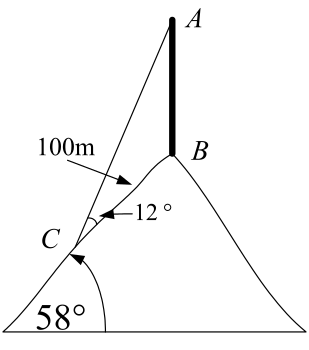
\includegraphics[ width=2.0851in, height=2.3575in,]{L4SZ2827}
}
%TCIMACRO{\TeXButton{End Two Columns}{\end {multicols}}}%
%BeginExpansion
\end {multicols}
%EndExpansion
 

\item [31.]
%TCIMACRO{\TeXButton{Start Two Columns}{\columnsep =30pt
% \begin {multicols}{2}}}%
%BeginExpansion
\columnsep =30pt
\begin {multicols}{2}
%EndExpansion
 A water tower $30 \mbox{m}$ tall is located at the top of a hill. From
a distance of $120 \mbox{m}$ down the hill it is observer that the angle formed between the top and
the base of the tower is $8 \mbox{{\ensuremath{{}^\circ}}}$. Find $\angle ABC\text{,}$ the angle of inclination of the hill. 

\item    
\setlength\fboxrule{0in}\setlength\fboxsep{0.2in}\fcolorbox[HTML]{000000}{FFFFFF}{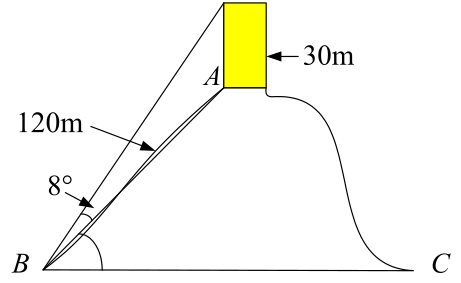
\includegraphics[ width=2.4829in, height=1.5281in,]{L4SZ2828}
}
%TCIMACRO{\TeXButton{End Two Columns}{\end {multicols}}}%
%BeginExpansion
\end {multicols}
%EndExpansion
 \end{description}

%\section{Excel Exercise}
%
%
%\subsection{The Sine Rule - Investigating the Ambiguous Case}
%In the notes we discussed the ambiguous case and we looked at the triangle $ \Delta A B C$. Given $A$, $a$ and $b$ we found two critical values of $a$ that determined whether there would be $0$, $1$ or $2$ solutions for the triangle. The results are summarised in the following table. 
%
%\qquad \qquad \qquad \qquad \qquad
%\begin{tabular}[c]{|c|l|}\hline
%$ <b \sin  A$  & $0$  \\
%\hline
%$ =b \sin  A$  & $1$ solution (right triangle)  \\
%\hline
%$b \sin  A <a <b$  & $2$ solutions  \\
%\hline
%$ =b$  & $1$ solution (one triangle is formed)  \\
%\hline
%$ >b$  & $1$ solution (second triangle invalid)  \\
%\hline
%\end{tabular}
%
%Let $A =30 \mbox{{\ensuremath{{}^\circ}}}$ and let $b =7$ 
%
%The task is to set out in a table the solutions for the triangle for the ambiguous case. (When
%there are 2 solutions.) 
%
%
%\begin{enumerate}
%\item Find the two values of $a$ that define the limits when two solutions are obtained. 
%
%\item Explore Excel
%to check you know how to use the \emph{sine} function. 
%
%\item In a column list values
%of $a$ with increments of $0.1\text{.}$ 
%
%\item Complete the first row of the table to give the two solutions.
%
%
%\item Use \textbf{Fill Down} to complete the table. 
%
%\item Inspect
%the table to ensure you are satisfied you understand the pattern produced. \end{enumerate}
%
%
%Look at the
%values for $c$ and explain why the value at the top of the column is half the value at the bottom. 
%
%Hints: 
%
%
%\begin{enumerate}
%\item Excel requires angles to be measured in radians so convert, (Use $A \times \pi  \div 180$). 
%
%\item To find B use $\sin ^{ -1} \genfrac{(}{)}{}{}{b \sin  A}{a}$. This angle is in radians so must now be converted to degrees. 
%
%\item To
%find $\sin ^{ -1}$ use the function a$\sin \text{.}$ (This is short for $\arcsin $ which is what Excel and some textbooks use for $\sin ^{ -1}\text{.}$) 
%
%\item To find $C$ use $180 -(A +B)$ 
%
%\item To find $c$ convert $A$ and $C$ to radians ($ \times 180 \div \pi $) and use $c =\frac{a \sin  C}{\sin  A}$ \end{enumerate}
%
%
%An example of the final result can be found below. 
%
%   
%\setlength\fboxrule{0.01in}\setlength\fboxsep{0.2in}\fcolorbox[HTML]{000000}{FFFFFF}{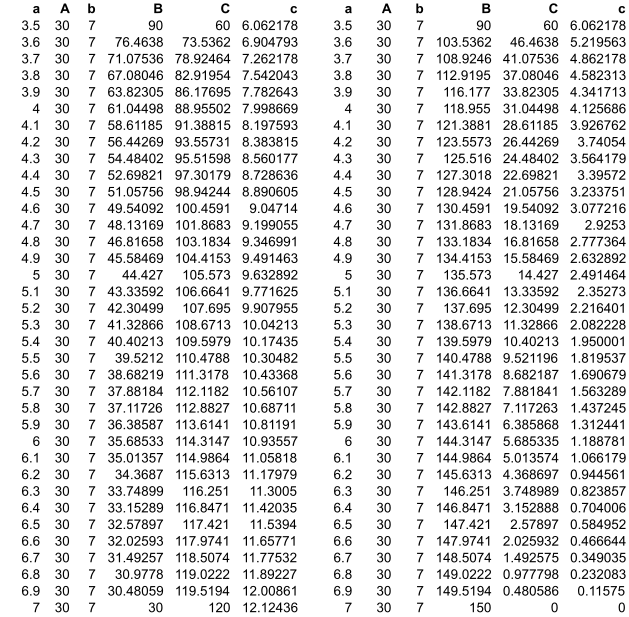
\includegraphics[ width=6.077in, height=5.9698in,]{L4SZ2829}
%}
%
%
%
%%TCIMACRO{\TeXButton{Start Two Columns}{\columnsep =30pt
%% \begin {multicols}{2}}}%
%%BeginExpansion
%\columnsep =30pt
%\begin {multicols}{2}
%%EndExpansion
% 
%
%
%%TCIMACRO{\TeXButton{End Two Columns}{\end {multicols}}}%
%%BeginExpansion
%\end {multicols}
%%EndExpansion
% 

\section{The Cosine Rule}


In this section we will state and prove the Cosine Rule (which is called "The Law of Cosines" in the
textbook). The proof is given here for completeness. You will not
be tested on your ability to reproduce it. The section will give examples where the Cosine Rule is used to solve
problems using the \emph{triangle of vectors} and we will include revision of \emph{bearings} and the use of trigonometry
in \emph{navigation}. 

In this course we have mentioned so far two formulae for the area of a triangle and many problems
allow us to use one of those two formulae. There is a third formula that is used when the three sides of the
triangle are given. In practical situations this is often the easiest and most likely data that has been collected
so this method might be the most useful of the three. The formula is named after the person who first derived
it. It is called \emph{Heron's Formula}. 

\subsection{Proof of The Cosine Rule}
\textbf{To prove:} For any triangle $ \Delta A B C\text{,}$ $a^{2} =b^{2} +c^{2} -2 b c \cos  A$  
%TCIMACRO{\TeXButton{Start Two Columns}{\columnsep =30pt
% \begin {multicols}{2}}}%
%BeginExpansion
\columnsep =30pt
\begin {multicols}{2}
%EndExpansion
 

\vspace{2cm}
\setlength\fboxrule{0in}\setlength\fboxsep{0.2in}\fcolorbox[HTML]{000000}{FFFFFF}{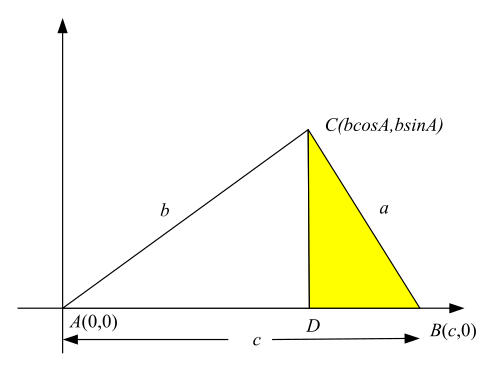
\includegraphics[ width=3.1021in, height=2.3549in,]{L4SZ282A}
}
By Pythagoras Theorem
\begin{align*}B C^{2} &  = C D^{2} +D B^{2} \\
a^{2} &  = \left (c -b \cos  A\right )^{2} +\left (b \sin  A\right )^{2} \\
 &  = c^{2} -2 b c \cos  A +b^{2} \cos ^{2} A +b^{2} \sin ^{2} A \\
 &  = c^{2} -2 b c \cos  A +b^{2} \left (\cos ^{2} A +\sin ^{2} A\right ) \\
 &  = c^{2} -2 b c \cos  A +b^{2}\text{as}\cos ^{2} A +\sin ^{2} A =1\text{\ }\end{align*} 
%TCIMACRO{\TeXButton{End Two Columns}{\end {multicols}}}%
%BeginExpansion
\end {multicols}
%EndExpansion
 

This is usually written
\begin{equation*}a^{2} =b^{2} +c^{2} -2 b c \cos  A
\end{equation*}

The diagram has been drawn to simplify the way the proof unfolds. You
will see that by placing the vertex $A$ at the origin the side $a$ is found in terms of $b$, $c$, and $A$. The proof would have been the same had $A$ and $B$ been as shown and $C$ placed in the second quadrant. (Thus producing a triangle with an obtuse angle at
$A$.) This rule is symmetrical. You need
to be given two sides and the included angle ($b$, $c$ and $A$) and the formula allows you to calculate $a$. Most textbooks will therefore show you three equivalent formulae
\begin{align*}a^{2} &  = b^{2} +c^{2} -2 b c \cos  A \\
b^{2} &  = c^{2} +a^{2} -2 c a \cos  B \\
c^{2} &  = a^{2} +b^{2} -2 a b \cos  C\end{align*}

In this course you will only be given one formula and you will have to know it is a reminder to
lay out your solution in this way. In particular to remind you where to put the plus and minus signs. 

\subsubsection{Example 1}
Given $a =5$, $b =6$ and $C =50 \mbox{{\ensuremath{{}^\circ}}}$, find $c$.
\begin{align*}c^{2} &  = a^{2} +b^{2} -2 a b \cos  C \\
 &  = 5^{2} +6^{2} -2 \times 5 \times 6 \times \cos  50 \mbox{{\ensuremath{{}^\circ}}} \\
 &  \approx   22.43274342 \\
c &  \approx   \sqrt{22.43274342} \\
 &  \approx   4.736321718 \approx 4.7 \left (1\text{dp}\right )\end{align*}

\subsubsection{Example 2}
Given $a =5$, $b =6$ and $C =130 \mbox{{\ensuremath{{}^\circ}}}$, find $c$.
\begin{align*}c^{2} &  = a^{2} +b^{2} -2 a b \cos  C \\
 &  = 5^{2} +6^{2} -2 \times 5 \times 6 \times \cos  130 \mbox{{\ensuremath{{}^\circ}}} \\
 &  \approx   99.56725658 \\
c &  \approx   \sqrt{99.56725658} \\
 &  \approx   9.97833937 \approx 10.0 \left (1\text{dp}\right )\end{align*}

These two examples show that when the two sides and the included angle are given the third side
(opposite the given angle) can be found. This is more useful when a practical example is given and example 1
p 513-514 talks about a surveyor using the Cosine Rule to measure the length of a tunnel. However when the problem
is analysed it is still just what we have covered in example 1 above. 

\subsection{To Find an Angle Given Three Sides}
The Cosine Rule states $a^{2} =b^{2} +c^{2} -2 b c \cos  A\text{.}$ So if $a$, $b$, and $c$ are given $A$ can be calculated. The formula can be rearranged as follows
\begin{align*}2 b c \cos  A &  = b^{2} +c^{2} -a^{2} \\
\cos  A &  = \frac{b^{2} +c^{2} -a^{2}}{2 b c}\end{align*}


\begin{enumerate}
\item Again to use this formula you must appreciate the symmetry and the pattern of the numbers otherwise you are
just blindly substituting in a formula without understanding. Notice the fact that the minus sign is in front
of the $a^{2}$ term and a is opposite the angle we are finding. 

\item Notice the $b$ and $c$ are the sides that include the angle we are finding and these sides appear in both the numerator and denominator. Because
of the symmetry of the result we can write
\begin{align*}\cos  A &  = \frac{b^{2} +c^{2} -a^{2}}{2 b c} \\
\cos  B &  = \frac{c^{2} +a^{2} -b^{2}}{2 c a} \\
\cos  C &  = \frac{a^{2} +b^{2} -c^{2}}{2 a b}\end{align*}\end{enumerate}


In this course you will be given one formula which
you should use by following the pattern it produces. 

\subsubsection{Example 3}
Given $a =5$, $b =6$ and $c =9$, find $A$. 

Because $a$ is the smallest side $A$ will most certainly be an acute angle.
\begin{align*}\cos  A &  = \frac{b^{2} +c^{2} -a^{2}}{2 b c} \\
 &  = \frac{6^{2} +9^{2} -5^{2}}{2 \times 6 \times 9} \\
 &  \approx 0.851851851 \\
A &  \approx \cos ^{ -1} \left (0.851851851\right ) \\
 &  \approx 31.6 \mbox{{\ensuremath{{}^\circ}}}\end{align*}

\subsubsection{Example 4}
For example 3 find $C$.
\begin{align*}\cos  C &  = \frac{a^{2} +b^{2} -c^{2}}{2 a b} \\
 &  = \frac{6^{2} +5^{2} -9^{2}}{2 \times 6 \times 5} \\
 &  \approx  -0. \dot{3} \\
C &  \approx \cos ^{ -1} \left ( -0. \dot{3}\right ) \\
 &  \approx 109.4712206 \\
 &  \approx 109.5 \mbox{{\ensuremath{{}^\circ}}}\end{align*}

\subsection{Navigation}
In a navigation question the direction is often given as a bearing. Thus $N 40 \mbox{{\ensuremath{{}^\circ}}} W$ is said "North $40 \mbox{{\ensuremath{{}^\circ}}}$ West" or "$40 \mbox{{\ensuremath{{}^\circ}}}$ West of North", and means start facing North and rotate $40 \mbox{{\ensuremath{{}^\circ}}}$ in a Westerly direction. A vector in this direction
is represented by an arrow. 

   
\setlength\fboxrule{0in}\setlength\fboxsep{0.2in}\fcolorbox[HTML]{000000}{FFFFFF}{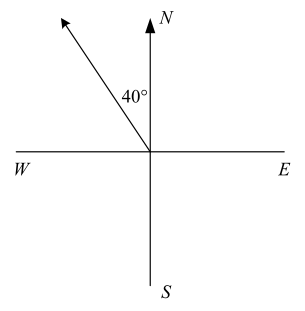
\includegraphics[ width=2.3817in, height=2.4284in,]{L4SZ282B}
}


A journey therefore can comprise a sequence of direction changes and potential speed changes. A
trap in these problems is to confuse distances and speeds. You must read your question carefully and make sure
that every vector on the diagram has been correctly converted so that they are all either distances or speeds. 

\subsubsection{Example}
A fisherman leaves his home port and heads in a direction $N 70 \mbox{{\ensuremath{{}^\circ}}} W$. He travels $48 \mbox{km}$ to reach his first fishing spot. The following
day he travels in a direction $N 10 \mbox{{\ensuremath{{}^\circ}}} E$ at $8 \mbox{km}$/$\mbox{h}$ for $10$ hours to reach his second fishing spot. 


\begin{description}
\item [(a)] How far is he from his home port when he arrives at his second
fishing spot? 

\item [(b)] What is the bearing of the home
port from his second fishing spot? 
\end{description}

The first journey is in $\mbox{km}$ so the second journey must be in $\mbox{km}$ too so that we can draw a triangle of vectors. $8 \mbox{km}$/$\mbox{h}$ for $10$ hours is $80 \mbox{km}$. Assume both journeys are in straight lines. 
\columnsep =30pt
\begin {multicols}{2}

\textbf{Strategy:}
\begin{enumerate}
\item [I] Make a reasonable sized diagram so that the NSEW axes can be placed at each
vertex of the triangle of vectors. 

\item [II] Don't forget about corresponding
angles and alternate angles because the NSEW axes create parallel lines. \end{enumerate}
    
\setlength\fboxrule{0in}\setlength\fboxsep{0.2in}\fcolorbox[HTML]{000000}{FFFFFF}{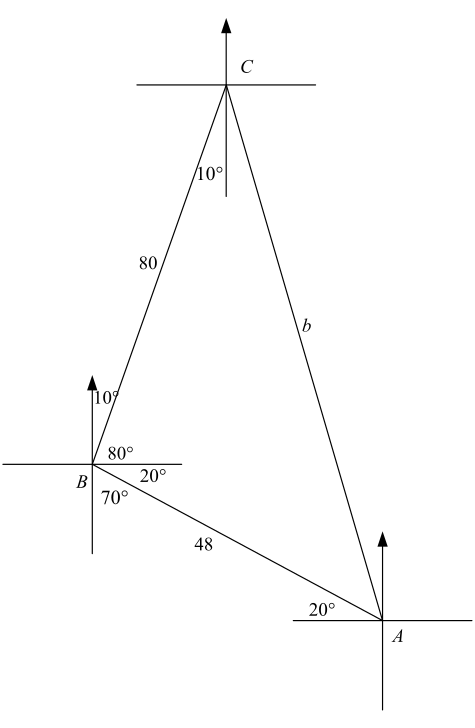
\includegraphics[ width=3.4817in, height=5.3082in,]{L4SZ282C}
}

\begin{enumerate}
\item Sketch the situation. 

\item Use your knowledge of parallel
lines to show the angle (between the two journeys) at $B$ is $100 \mbox{{\ensuremath{{}^\circ}}}$. 

\item (a) You have two sides ($48$ and $80$) and the included angle ($100 \mbox{{\ensuremath{{}^\circ}}}$) so the\ Cosine Rule can be used to find $A C$ the journey back to port.
\begin{align*}b^{2} &  = c^{2} +a^{2} -2 c a \cos  B \\
 &  = 48^{2} +80^{2} -2 \times 48 \times 80 \times \cos  100 \mbox{{\ensuremath{{}^\circ}}} \\
 &  \approx   10037.618 \\
b &  \approx   100.1879135 \approx 100 \mbox{km}\end{align*}

\item (b) To find the bearing you must first find another angle
in the triangle. Find $C$. (Use the Sine Rule or Cosine Rule - both should work.)
\begin{align*}\frac{\sin  C}{c} &  = \frac{\sin  B}{b} \\
\sin  C &  = \frac{c \sin  B}{b} \\
 &  \approx   \frac{48 \sin  100 \mbox{{\ensuremath{{}^\circ}}}}{100} \\
 &  \approx   0.472707721 \\
C &  \approx   \sin ^{ -1} 0.472707721 \\
 &  \approx   28.21020463 \mbox{{\ensuremath{{}^\circ}}} \approx 28 \mbox{{\ensuremath{{}^\circ}}}\end{align*}\end{enumerate}



%TCIMACRO{\TeXButton{End Two Columns}{\end {multicols}}}%
%BeginExpansion
\end {multicols}
%EndExpansion


Put the $28 \mbox{{\ensuremath{{}^\circ}}}$ on the diagram and show that the angle between the vertical and the journey back to port
is $18 \mbox{{\ensuremath{{}^\circ}}}$. Bearing from South is $S 18 \mbox{{\ensuremath{{}^\circ}}} E\text{.}$ Bearing from North is $N 162 \mbox{{\ensuremath{{}^\circ}}} E$ 

\subsection{The Area of Triangle using Heron's Formula}
In this section we show you Heron's Formula to find the area of a triangle given the three sides. We
will then have three formulae that you could use and each requires different facts to be given. 


\begin{tabular}[c]{|l|l|}\hline
\textbf{Given}
& \textbf{Area}  \\
\hline
Base and height
& $\frac{1}{2} \times $ base $ \times $ height  \\
\hline
2 sides and the included angle
($a$,$b$ and $C$)  & $\frac{1}{2} a b \sin  C$  \\
\hline
3 sides ($a$, $b$ and $c$)  & $\sqrt{s \left (s -a\right ) \left (s -b\right ) \left (s -c\right )}$ where $s =\frac{1}{2} \left (a +b +c\right )$  \\
\hline
\end{tabular}

$s$ is called the \emph{semiperimeter}. 

We will not discuss this proof in this course. Heron's
formula is very useful because you are more likely in practice to be required to find the area of a triangle whose sides are given than being given the
base and height or two sides and the included angle. 

\subsubsection{Example}
Given a triangle whose sides are $9 \mbox{cm}$, $10 \mbox{cm}$, and $11 \mbox{cm}$, find its area.
\begin{align*}s &  = \frac{1}{2} \left (9 +10 +11\right ) \\
 &  = 15 \\
\text{Area} &  = \sqrt{15 (15 -9) (15 -10) (15 -11)} \\
 &  = \sqrt{15 \times 6 \times 5 \times 4} \\
 &  \approx 42.42640687 \approx 42 cm^{2}\end{align*}

\subsection{Exercises}
The following exercises from pp 518-521 have been covered in this section: 


\begin{description}
\item [1.]   
%TCIMACRO{\TeXButton{Start Two Columns}{\columnsep =30pt
% \begin {multicols}{2}}}%
%BeginExpansion
\columnsep =30pt
\begin {multicols}{2}
%EndExpansion
 Use the Cosine Rule to find $x$ 

\item    
\setlength\fboxrule{0in}\setlength\fboxsep{0.2in}\fcolorbox[HTML]{000000}{FFFFFF}{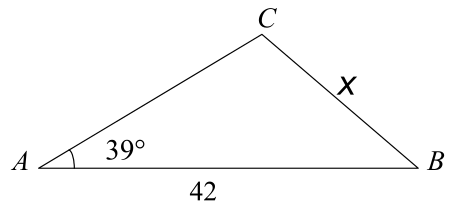
\includegraphics[ width=2.8236in, height=1.3007in,]{L4SZ282D}
}
\vspace*{1.5cm} 

\item [5.]
Use the Cosine Rule to find $\theta $ 

\item    
\setlength\fboxrule{0in}\setlength\fboxsep{0.2in}\fcolorbox[HTML]{000000}{FFFFFF}{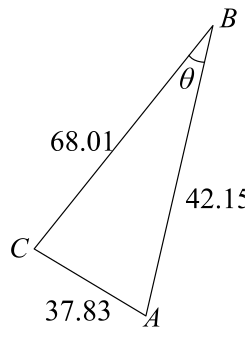
\includegraphics[ width=1.2747in, height=1.7262in,]{L4SZ282E}
}
%TCIMACRO{\TeXButton{End Two Columns}{\end {multicols}}}%
%BeginExpansion
\end {multicols}
%EndExpansion
 \end{description}

Solve the triangle ABC for questions 9, 13, and 15. 


\begin{description}
\item [9.]    
\setlength\fboxrule{0in}\setlength\fboxsep{0.2in}\fcolorbox[HTML]{000000}{FFFFFF}{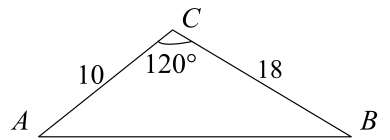
\includegraphics[ width=2.693in, height=0.9798in,]{L4SZ282F}
}


\item [13.] $a =20\text{,}$ $b =25\text{,}$ $c =22$ 

\item [15.] $b =125\text{,}$ $c =162\text{,}$ $\angle B =40 \mbox{{\ensuremath{{}^\circ}}}$ \end{description}

For questions 19 and 23 use either the Sine Rule or Cosine
Rule as appropriate. 


\begin{description}
\item [19.]   
%TCIMACRO{\TeXButton{Start Two Columns}{\columnsep =30pt
% \begin {multicols}{2}}}%
%BeginExpansion
\columnsep =30pt
\begin {multicols}{2}
%EndExpansion
    
\setlength\fboxrule{0in}\setlength\fboxsep{0.2in}\fcolorbox[HTML]{000000}{FFFFFF}{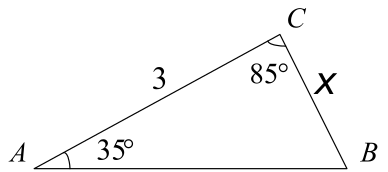
\includegraphics[ width=2.5166in, height=1.1234in,]{L4SZ282G}
}


\item [23.]    
\setlength\fboxrule{0in}\setlength\fboxsep{0.2in}\fcolorbox[HTML]{000000}{FFFFFF}{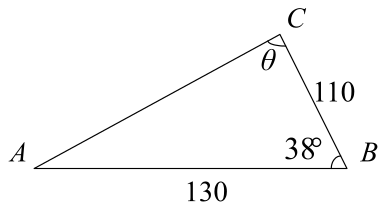
\includegraphics[ width=2.412in, height=1.3309in,]{L4SZ282H}
}
%TCIMACRO{\TeXButton{End Two Columns}{\end {multicols}}}%
%BeginExpansion
\end {multicols}
%EndExpansion
 

\item [27.]
%TCIMACRO{\TeXButton{Start Two Columns}{\columnsep =30pt
% \begin {multicols}{2}}}%
%BeginExpansion
\columnsep =30pt
\begin {multicols}{2}
%EndExpansion
 To find the distance across a small lake, a surveyor has taken the measurements shown. Find
the distance across the lake using this information. 

\item    
\setlength\fboxrule{0in}\setlength\fboxsep{0.2in}\fcolorbox[HTML]{000000}{FFFFFF}{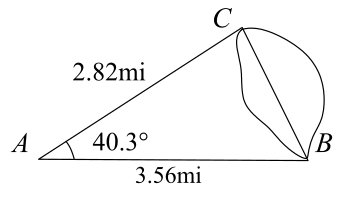
\includegraphics[ width=2.7665in, height=1.5965in,]{L4SZ282I}
}
%TCIMACRO{\TeXButton{End Two Columns}{\end {multicols}}}%
%BeginExpansion
\end {multicols}
%EndExpansion
 

\item [29.]
Two straight roads diverge at an angle of $65 \mbox{{\ensuremath{{}^\circ}}}$. Two cars leave the intersection at $2.00$ P.M., one traveling at $50 mi/\mbox{h}$ and the other at $30 mi/\mbox{h}$. How far apart are the cars at $2.30$ P.M.? 

\item [31.] A pilot flies
in a straight path for $1 \mbox{h}\; 30 \mbox{min}$. She then makes a course correction, heading $10 \mbox{{\ensuremath{{}^\circ}}}$ to the right of her original course, and flies for $2 \mbox{h}$ in the new direction. If she
maintains a constant speed of $625 mi/\mbox{h}$ how far is she from her starting point? 

\item [33.]
A fisherman leaves his home port and heads in a direction N $70 \mbox{{\ensuremath{{}^\circ}}}$ W. he travels $30 \mbox{mi}$ and reaches Egg Island. The next day he sails N
$10 \mbox{{\ensuremath{{}^\circ}}}$ E for $50 \mbox{mi}$, reaching Forrest Island. 

\item [(a)]
Find the distance between the fisherman's home port and Forrest Island. 

\item [(b)]
Find the bearing from Forrest Island back to his home port. 

\item [35.]
A triangular field has sides of lengths $22$, $36$, and $44$ yd. Find the largest angle. 

\item [37.]
A boy is flying two kites at the same time. He has $380 \mbox{ft}$ of line out to one kite and $420 \mbox{ft}$ of line out to the other. He estimates the angle
between the two lines is $30 \mbox{{\ensuremath{{}^\circ}}}$. Find the approximate distance between the two
kites. 

\item [39.]   
%TCIMACRO{\TeXButton{Start Two Columns}{\columnsep =30pt
% \begin {multicols}{2}}}%
%BeginExpansion
\columnsep =30pt
\begin {multicols}{2}
%EndExpansion
 A steep mountain is inclined $74 \mbox{{\ensuremath{{}^\circ}}}$ to the horizontal and rises $3400 \mbox{ft}$ above the surrounding plain. A cable car is to
be installed from a point $800 \mbox{ft}$ from the base to the top of the mountain, as shown. Find
the shortest length of cable needed. 

\item    
\setlength\fboxrule{0in}\setlength\fboxsep{0.2in}\fcolorbox[HTML]{000000}{FFFFFF}{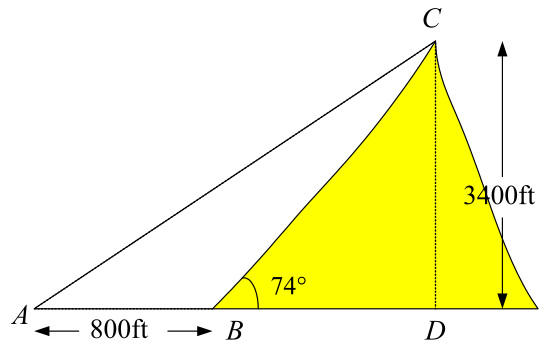
\includegraphics[ width=2.4587in, height=1.5912in,]{L4SZ282J}
}
%TCIMACRO{\TeXButton{End Two Columns}{\end {multicols}}}%
%BeginExpansion
\end {multicols}
%EndExpansion
 \end{description}


\begin{description}
\item [41.] Three circles of radii $4$, $5$, and $6 \mbox{cm}$ respectively are mutually tangent. Find the area
enclosed between the circles. 

\item \qquad \qquad \qquad \qquad
\setlength\fboxrule{0in}\setlength\fboxsep{0.2in}\fcolorbox[HTML]{000000}{FFFFFF}{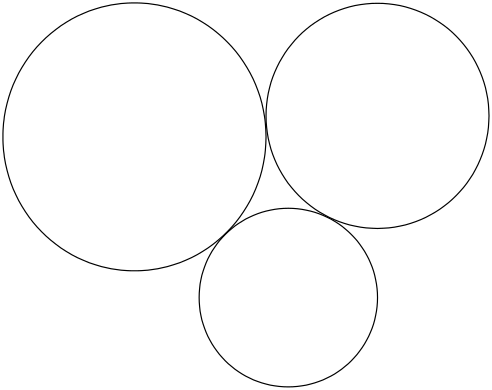
\includegraphics[ width=3.3269in, height=2.6394in,]{L4SZ282K}
}


\item [43.]   
%TCIMACRO{\TeXButton{Start Two Columns}{\columnsep =30pt
% \begin {multicols}{2}}}%
%BeginExpansion
\columnsep =30pt
\begin {multicols}{2}
%EndExpansion
 A surveyor wishes to find the distance between two points $A$ and $B$ on the opposite side of a river. on her side of the river she chooses two points
$C$ and $D$ that are $20 \mbox{m}$ apart and measures the angles shown. Find
the distance between $A$ and $B\text{.}$ 

\item    
\setlength\fboxrule{0in}\setlength\fboxsep{0.2in}\fcolorbox[HTML]{000000}{FFFFFF}{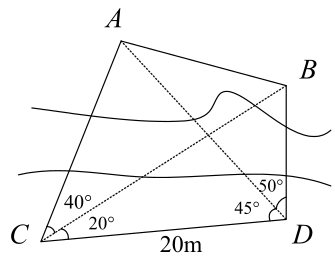
\includegraphics[ width=2.5028in, height=1.9995in,]{L4SZ282L}
}
%TCIMACRO{\TeXButton{End Two Columns}{\end {multicols}}}%
%BeginExpansion
\end {multicols}
%EndExpansion
 

\item [45.]
Land in downtown Columbia is valued at $ \$20$ a square foot. What is the value of a triangular lot with sides of lengths $112$, $148$, and $190 \mbox{ft}$? \end{description}


%TCIMACRO{\TeXButton{Start Two Columns}{\columnsep =30pt
% \begin {multicols}{2}}}%
%BeginExpansion
\columnsep =30pt
\begin {multicols}{2}
%EndExpansion
 


%TCIMACRO{\TeXButton{End Two Columns}{\end {multicols}}}%
%BeginExpansion
\end {multicols}
%EndExpansion
 

\section{Answers}
%TCIMACRO{\TeXButton{Start Two Columns}{\columnsep =30pt
% \begin {multicols}{2}}}%
%BeginExpansion
\columnsep =30pt
\begin {multicols}{2}
%EndExpansion
 

\textbf{Exercises 3.1} 

1. $\frac{\pi }{5} \approx 0.628 \mbox{rad}$ 

3. $\frac{ -8 \pi }{3} \approx  -8.378 \mbox{rad}$ 

5. $\frac{\pi }{3} \approx 1.047 \mbox{rad}$ 

7. $\frac{ -3 \pi }{4} \approx  -2.356 \mbox{rad}$ 

9. $135 \mbox{{\ensuremath{{}^\circ}}}$ 

11. $150 \mbox{{\ensuremath{{}^\circ}}}$ 

13. $\frac{ -270}{\pi } \approx  -85.9 \mbox{{\ensuremath{{}^\circ}}}$ 

15. $ -15 \mbox{{\ensuremath{{}^\circ}}}$ 

41. $\frac{55 \pi }{9} \approx 19.2$ 

43. $4$ 

45. $4 \mbox{mi}$ 

47. $2 \mbox{rad} \approx 114.6 \mbox{{\ensuremath{{}^\circ}}}$ 

49. $\frac{36}{\pi } \approx 11.459 \mbox{m}$ 

51. $330 \pi  \approx 1037 \mbox{mi}$ 

53. $1.6$ million $\mbox{mi}$ 

55. $1.15 \mbox{mi}$ 

57. $50 \mathrm{m}^{2}$ 

59. $4 \mbox{m}$ 

61. $6 cm^{2}$ 

63. $\frac{32 \pi }{15} ft/\mbox{s}$ 

65.(a) $2000 \pi  rad/\mbox{min}$ (b) $\frac{50 \pi }{3} ft/\mbox{s} \approx 52.4 ft/\mbox{s}$ 

67. $39.3 mi/\mbox{h}$ 

69. $2.1 \mathrm{m}/\mbox{s}$ 

\textbf{Exercises 3.2} 

1. $\sin  \theta  =\frac{4}{5} ,\cos  \theta  =\frac{3}{5} ,\tan  \theta  =\frac{4}{3}$ 

3. $\sin  \theta  =\frac{40}{41} ,\cos  \theta  =\frac{9}{41} ,\tan  \theta  =\frac{40}{9}$ 

5. $\sin  \theta  =\frac{2 \sqrt{13}}{13} ,\cos  \theta  =\frac{3 \sqrt{13}}{13} ,\tan  \theta  =\frac{2}{3}$ 

10. $12 \sqrt{2}$ 

11. $\frac{13 \sqrt{3}}{2}$ 

13. $16.51658$ 

29. $45 \mbox{{\ensuremath{{}^\circ}}} ,16 ,16 \sqrt{2} \approx 22.63$ 

31. $38 \mbox{{\ensuremath{{}^\circ}}} ,44.79 ,56.85$ 

35. $1026 \mbox{ft}$ 

37.(a) $2100 \mbox{mi}$ (b) No 

39. $19 \mbox{ft}$ 

42. $600 \sin  65 \mbox{{\ensuremath{{}^\circ}}} \approx 544 \mbox{ft}$ 

43. $345 \mbox{ft}$ 

45. $415 \mbox{ft} ,152 \mbox{ft}$ 

46.$11,379 \mbox{ft}$ 

49. $5808 \mbox{ft}$ 

\textbf{Exercises 3.3} 

7. $\frac{1}{2}$ 

9. $ -\frac{\sqrt{2}}{2}$ 

11. $ -\sqrt{3}$ 

15. $ -\frac{\sqrt{3}}{2}$ 

17. $\frac{\sqrt{3}}{3}$ 

19. $\frac{\sqrt{3}}{2}$ 

21. $ -1$ 

23. $\frac{1}{2}$ 

29. undefined 

41. $\cos  \theta  = -\frac{4}{5} ,\tan  \theta  = -\frac{3}{4}$ 

43. $\sin  \theta  = -\frac{3}{5} ,\cos  \theta  =\frac{4}{5}$ 

49. (a) $\frac{\sqrt{3}}{2} ,\sqrt{3}$ (b) $\frac{1}{2} ,\frac{\sqrt{3}}{4}$ (c) $\frac{3}{4} ,0.88967$ 

51. $19.1$ 

53. $66.1 \mbox{{\ensuremath{{}^\circ}}}$ 

\textbf{Exercises 3.4} 

1. $318.8$ 

5. $44 \mbox{{\ensuremath{{}^\circ}}}$ 

7. $\angle C =114 \mbox{{\ensuremath{{}^\circ}}} ,a \approx 51 ,b \approx 24$ 

9. $\angle C =62 \mbox{{\ensuremath{{}^\circ}}} ,a \approx 200 b \approx 242$ 
%TCIMACRO{\TeXButton{End Two Columns}{\end {multicols}}}%
%BeginExpansion

%EndExpansion
  

13. $\angle A =100 \mbox{{\ensuremath{{}^\circ}}} ,a \approx 89 ,c \approx 71$ 

15. $\angle B \approx 30 \mbox{{\ensuremath{{}^\circ}}} ,\angle C \approx 40 \mbox{{\ensuremath{{}^\circ}}} ,c \approx 19$ 

17. no solution 

19. $\angle A_{1} \approx 125 \mbox{{\ensuremath{{}^\circ}}} ,\angle C_{1} \approx 30 \mbox{{\ensuremath{{}^\circ}}} ,a_{1} \approx 49\text{,}$ 

\  \ $\angle A_{2} \approx 5 \mbox{{\ensuremath{{}^\circ}}} ,\angle C_{2} \approx 150 \mbox{{\ensuremath{{}^\circ}}} ,a_{2} \approx 5.6$ 

23. $219 \mbox{ft}$ 

25. (b) $1018 \mbox{mi}\text{,}$ (c) $1017 \mbox{mi}$ 

27. $155 \mbox{m}$ 

31. $48.2 \mbox{{\ensuremath{{}^\circ}}}$ 

\textbf{Exercises 3.5} 

1. $28.9$ 

5. $29.89 \mbox{{\ensuremath{{}^\circ}}}$ 

9. $\angle A \approx 39.4 \mbox{{\ensuremath{{}^\circ}}} ,\angle B \approx 20.6 \mbox{{\ensuremath{{}^\circ}}} ,c \approx 24.6$ 

13. $\angle A \approx 50 \mbox{{\ensuremath{{}^\circ}}} ,\angle B \approx 73 \mbox{{\ensuremath{{}^\circ}}} ,\angle C \approx 57 \mbox{{\ensuremath{{}^\circ}}}$ 

15. $\angle A_{1} \approx 83.6 \mbox{{\ensuremath{{}^\circ}}} ,\angle C_{1} \approx 56.4 \mbox{{\ensuremath{{}^\circ}}} ,a_{1} \approx 193$ 

\  \ $\angle A_{2} \approx 16.4 \mbox{{\ensuremath{{}^\circ}}} ,\angle C_{2} \approx 123.6 \mbox{{\ensuremath{{}^\circ}}} ,a_{2} \approx 54.9$ 

19. $2$ 

23. $84.6 \mbox{{\ensuremath{{}^\circ}}}$ 

27. $2.30 \mbox{mi}$ 

29. $23.1 \mbox{mi}$ 

31 $2179 \mbox{mi}$ 

33. (a) $62.6 \mbox{mi}$ (b) $S 18.2 \mbox{{\ensuremath{{}^\circ}}} E$ 

35. $96 \mbox{{\ensuremath{{}^\circ}}}$ 

37. $211 \mbox{ft}$ 

39. $3835 \mbox{ft}$ 

41. $3.85 cm^{2}$ 

43. $14.3 \mbox{m}$ 

45. $ \$165,554$ 

\end {multicols}

\section{Trigonometric Functions of Real Numbers}
In this next part of the chapter the three main trigonometric functions (sine, cosine and tangent) will be studied. They
will be viewed as functions of real numbers. This means that the domains of the functions are the real numbers.
The first half viewed the functions in terms of angles. This
means that the domains of the functions will be angles. The trigonometric functions defined in these two ways
are identical and there is a simple rule connecting the domains. Why do we show you the two approaches? Trigonometry
will be used to solve a variety of problems and these can be divided into two groups, dynamic problems and static problems. When
dynamic problems (such as problems involving motion) are being solved real numbers will be used. When
static problems (such as finding distances and angles for triangles) are being solved angles will be used. 

\section{The Unit Circle}
In this session frequent reference will be made to the measurement of distances around the perimeter
of the unit circle. The unit circle is defined as a circle centre $\left (0 ,0\right )$ radius $1$. Its equation is $x^{2} +y^{2} =1$. In mathematics we are always on the lookout for patterns that make our calculations
easier. for instance, recently we discussed the circle $x^{2} +y^{2} =25$. (Circle centre $\left (0 ,0\right )$ radius $5$.) We found the point $\left (3 ,4\right )$ was on the circle ($3^{2} +4^{2} =5^{2}$). The unit circle also has some patterns that you should become familiar with. 

\subsubsection{Example}
Show $\left (\frac{\sqrt{2}}{2} ,\frac{\sqrt{2}}{2}\right )$ is on the unit circle. 

Because we are given
the coordinates of the point we are required to show that $x^{2} +y^{2} =1$. 

$x^{2} +y^{2} =\genfrac{(}{)}{}{}{\sqrt{2}}{2}^{2} +\genfrac{(}{)}{}{}{\sqrt{2}}{2}^{2} =\frac{2}{4} +\frac{2}{4} =\frac{1}{2} +\frac{1}{2} =1$ 

So $x^{2} +y^{2} =1$ proves that $\left (\frac{\sqrt{2}}{2} ,\frac{\sqrt{2}}{2}\right )$ lies on the unit circle. 

\subsubsection{Example}
Given $\left (\frac{1}{2} ,a\right )$ lies on the unit circle find $a$. 

Because we are told the point lies on the unit circle we substitute
\begin{align*}\genfrac{(}{)}{}{}{1}{2}^{2} +a^{2} &  = 1 \\
	\frac{1}{4} +a^{2} &  = 1 \\
	a^{2} &  = 1 -\frac{1}{4} =\frac{3}{4} \\
	a &  =  \pm \sqrt{\frac{3}{4}} = \pm \frac{\sqrt{3}}{\sqrt{4}} = \pm \frac{\sqrt{3}}{2}\end{align*}

This means there are two possible solutions $\left (\frac{1}{2} ,\frac{\sqrt{3}}{2}\right )$ and $\left (\frac{1}{2} , -\frac{\sqrt{3}}{2}\right )$. A diagram will show
this to you. Notice the right angled triangle we can draw to produce the result. 


\subsection{Terminal Points}
An important skill we require in this section is to be able to connect the coordinates of a point on the unit circle with a length on the circumference
of the unit circle. For this we have a convention. \emph{All
	distances are measured anticlockwise from the point }$\left (1 ,0\right )$. (Books may use
the word counterclockwise in place of anticlockwise. These words are used interchangeably.) In
the digital world of today these terms are not as widely used as they were when only analog clocks had been invented. We
find them convenient words to use because they explain precisely what we want to say. 

We let $t$ be the distance to a point on the unit circle from the point $\left (1 ,0\right )$. $t$ is a real number so distances that are measured in an anticlockwise direction are positive and distances measured in a clockwise
direction are negative. 

\textbf{Definition:} When you measure a distance of $t$ around the perimeter of the unit circle and arrive at a point $P (x ,y)$ the point $P (x ,y)$ is defined as a \emph{terminal point}.

Some terminal points are easy to find provided you remember how to find the perimeter of the unit circle.
\begin{align*}\text{Perimeter} &  = 2 \pi  r\text{\  but if}r =1 \\
	&  = 2 \pi  \times 1 =2 \pi \end{align*}

This means that if you measure from $\left (1 ,0\right )$ right around the unit circle to the starting point $t =2 \pi $. So if $t =2 \pi $ the terminal point is $\left (1 ,0\right )$. 

\subsubsection{Example}
Find the coordinates of the terminal point when (a) $t =\pi $ (b) $t =5 \pi $ (c) $t =\frac{ -3 \pi }{2}$ 

Terminal points are obtained from a sketch of the situation. 

(a) $\left ( -1 ,0\right )$ (b) $\left ( -1 ,0\right )$ (c) $\left (0 ,1\right )$ 

There are other values we will use
that are more easily deduced once chapter 6 in the textbook has been completed. At this stage it is easier to
state these in a table and focus on using the values obtained to solve other related problems. 

We give the terminal point for $0$, $\frac{\pi }{6}$, $\frac{\pi }{4}$, $\frac{\pi }{3}$ and $\frac{\pi }{2}$. 


\begin{tabular}[c]{|r|l|l|l|l|l|}\hline
	$t$  & $0$  & $\frac{\pi }{6}$  & $\frac{\pi }{4}$  & $\frac{\pi }{3}$  & $\frac{\pi }{2}$  \\
	\hline
	Terminal Point  & $\left (1 ,0\right )$  & $\left (\frac{\sqrt{3}}{2} ,\frac{1}{2}\right )$  & $\left (\frac{\sqrt{2}}{2} ,\frac{\sqrt{2}}{2}\right )$  & $\left (\frac{1}{2} ,\frac{\sqrt{3}}{2}\right )$  & $\left (0 ,1\right )$  \\
	\hline
\end{tabular}

These will be given if required in a test. 

\subsubsection{Example}
Use the table to find the terminal points for (a) $t =\frac{5 \pi }{3}$ (b) $t =\frac{ -7 \pi }{6}$ 

(a) $\left (\frac{1}{2} ,\frac{ -\sqrt{3}}{2}\right )$ (b) $\left (\frac{ -\sqrt{3}}{2} ,\frac{1}{2}\right )$ 

Examples 3 and 4 pp 411-413 are about finding
terminal points. 

\subsection{Reference Numbers}
A useful way to connect the terminal point with the distance around the unit circle $t$ is to define a further quantity, the \emph{reference number} $\bar{t}$. However if you understand how to relate a particular value of $t$ with an appropriate value in the first quadrant to allow you to use the table then the need for the definition of a reference
number may be unnecessary. In this course we will tackle problems using the approach given in example 4 above
until the need to define the reference number is unavoidable. 

\subsection{Exercises}
Show that the point is on the unit circle. 


\begin{description}
	\item [1.]   
	%TCIMACRO{\TeXButton{Start Two Columns}{\columnsep =30pt
	% \begin {multicols}{2}}}%
	%BeginExpansion
	\columnsep =30pt
	\begin {multicols}{2}
	%EndExpansion
	$\left (\frac{3}{5} ,\frac{4}{5}\right )$ 
	
	\item [3.]
	$\left ( -\frac{2}{3} , -\frac{\sqrt{5}}{3}\right )$ 
	%TCIMACRO{\TeXButton{End Two Columns}{\end {multicols}}}%
	%BeginExpansion
	\end {multicols}
	%EndExpansion
\end{description}

The point $P$ is on the unit circle. Find $P (x ,y)$ from the given information. 


\begin{description}
	\item [5.] The $x$-coordinate of $P$ is $\frac{4}{5}$ and $P$ is in quadrant I. 
	
	\item [7.] The
	$y$-coordinate of of $P$ is $\frac{2}{3}$ and the $x$-coordinate is negative. 
	
	\item [9.]
	The $x$-coordinate of $P$ is $ -\sqrt{2}/3$ and $P$ is in quadrant III. \end{description}

Find the terminal point $P (x ,y)$ on the unit circle determined by the given value of $t$. 


\begin{description}
	\item [13.]   
	%TCIMACRO{\TeXButton{Start Two Columns}{\columnsep =30pt
	% \begin {multicols}{2}}}%
	%BeginExpansion
	\columnsep =30pt
	\begin {multicols}{2}
	%EndExpansion
	$t =\frac{\pi }{2}$ 
	
	\item [15.] $t =\frac{5 \pi }{6}$ 
	%TCIMACRO{\TeXButton{End Two Columns}{\end {multicols}}}%
	%BeginExpansion
	\end {multicols}
	%EndExpansion
	
	
	\item [17.]
	%TCIMACRO{\TeXButton{Start Two Columns}{\columnsep =30pt
	% \begin {multicols}{2}}}%
	%BeginExpansion
	\columnsep =30pt
	\begin {multicols}{2}
	%EndExpansion
	$t = -\frac{\pi }{3}$ 
	
	\item [19.] $t =\frac{2 \pi }{3}$ 
	%TCIMACRO{\TeXButton{End Two Columns}{\end {multicols}}}%
	%BeginExpansion
	\end {multicols}
	%EndExpansion
	
	
	\item [21.]
	$t = -\frac{3 \pi }{4}$ 
	
	\item [23.] Suppose that the terminal
	point determined by $t$ is the point $\left (\frac{3}{5} ,\frac{4}{5}\right )$ on the unit circle. Find
	the terminal point determined by each of the following. 
	
	\item [(a)]
	%TCIMACRO{\TeXButton{Start Two Columns}{\columnsep =30pt
	% \begin {multicols}{2}}}%
	%BeginExpansion
	\columnsep =30pt
	\begin {multicols}{2}
	%EndExpansion
	$\pi  -t$ 
	
	\item [(b)] $ -t$ 
	%TCIMACRO{\TeXButton{End Two Columns}{\end {multicols}}}%
	%BeginExpansion
	\end {multicols}
	%EndExpansion
	
	
	\item [(c)]
	%TCIMACRO{\TeXButton{Start Two Columns}{\columnsep =30pt
	% \begin {multicols}{2}}}%
	%BeginExpansion
	\columnsep =30pt
	\begin {multicols}{2}
	%EndExpansion
	$\pi  +t$ 
	
	\item [(d)] $t -\pi $ 
	%TCIMACRO{\TeXButton{End Two Columns}{\end {multicols}}}%
	%BeginExpansion
	\end {multicols}
	%EndExpansion
\end{description}


%TCIMACRO{\TeXButton{Start Two Columns}{\columnsep =30pt
% \begin {multicols}{2}}}%
%BeginExpansion
\columnsep =30pt
\begin {multicols}{2}
%EndExpansion



%TCIMACRO{\TeXButton{End Two Columns}{\end {multicols}}}%
%BeginExpansion
\end {multicols}
%EndExpansion

\section{The Trigonometric Functions of Real Numbers}
In this section we define sine, cosine and tangent based on $t$ as defined in section $7.1$. You need to be very careful to decide which quadrant the terminal point is in
so that the signs of the trigonometric functions are correct. 

\textbf{Definitions:} Given a real number $t$. If we move a distance $t$ around the unit circle starting at the point $\left (1 ,0\right )$ and we arrive at a point $P (x ,y)$ then $x =\cos  t$, $y =\sin  t$ and $\frac{y}{x} =\tan  t$ $\left (x \neq 0\right )$. 

A sketch will show the relationship between
$t$, $x$, and $y$. 

A fundamental relationship between sine, cosine and tangent comes from these definitions
\begin{equation*}\tan  t =\frac{\sin  t}{\cos  t}
\end{equation*}

We call this relationship an \emph{identity} because it is true for all values
of $t$. 

There are six trigonometric functions. The other three are
secant, cosecant and cotangent. The are sometimes referred to as the reciprocal functions because: 

Secant is defined by $\sec  t =\frac{1}{\cos  t} =\frac{1}{x}$ 

Cosecant is defined by co$\sec  t =\frac{1}{\sin  t} =\frac{1}{y}$ ($ =$csc $t$) 

Cotangent is defined by $\cot  t =\frac{1}{\tan  t} =\frac{x}{y}$ $\left (y \neq 0\right )$ 

In this course we will focus on sine, cosine
and tangent and only use secant, cosecant and cotangent when it is unavoidable. 

The table in section 7.1 can now be extended to include
sine, cosine and tangent. 

\qquad \qquad
\begin{tabular}[c]{|c|c|c|c|c|}\hline
	$t$  & Terminal Point  & $x =\cos  t$  & $y =\sin  t$  & $\frac{y}{x} =\tan  t$  \\
	\hline
	$0$  & $\left (1 ,0\right )$  & $1$  & $0$  & $\frac{0}{1} =0$  \\
	\hline
	$\frac{\pi }{6}$  & $\left (\frac{\sqrt{3}}{2} ,\frac{1}{2}\right )$  & $\frac{\sqrt{3}}{2}$  & $\frac{1}{2}$  & $\frac{1}{2} \div \frac{\sqrt{3}}{2} =\frac{1}{2} \times \frac{2}{\sqrt{3}} =\frac{1}{\sqrt{3}} =\frac{\sqrt{3}}{3}$  \\
	\hline
	$\frac{\pi }{4}$  & $\left (\frac{\sqrt{2}}{2} ,\frac{\sqrt{2}}{2}\right )$  & $\frac{\sqrt{2}}{2}$  & $\frac{\sqrt{2}}{2}$  & $\frac{\sqrt{2}}{2} \div \frac{\sqrt{2}}{2} =1$  \\
	\hline
	$\frac{\pi }{3}$  & $\left (\frac{1}{2} ,\frac{\sqrt{3}}{2}\right )$  & $\frac{1}{2}$  & $\frac{\sqrt{3}}{2}$  & $\frac{\sqrt{3}}{2} \div \frac{1}{2} =\frac{\sqrt{3}}{2} \times \frac{2}{1} =\sqrt{3}$  \\
	\hline
	$\frac{\pi }{2}$  & $\left (0 ,1\right )$  & $0$  & $1$  & $\frac{1}{0}$ undefined $\left ( =\infty \right )$  \\
	\hline
\end{tabular}

Should you be asked about secant, cosecant or cotangent you should look up the respective reciprocal relationship and calculate it from that.


\subsubsection{Values of Trigonometric Functions}
The value of a trigonometric function consists of two parts the numerical part and the sign. you
must get both parts correct. In the previous section (example 4) you related the values of a terminal point
to another point in the first quadrant. A point on the unit circle could be in any one of the four quadrants.
\ You should develop an intuitive understanding of how this allows you to be sure of the sign of your answer.


\qquad \qquad \qquad \qquad
\begin{tabular}[c]{|c|c|c|c|c|c|}\hline
	Quadrant  & $x$-coordinate  & $y$-coordinate  & $\cos $  & $\sin $  & $\tan $  \\
	\hline
	$1$  & $ +$  & $ +$  & $ +$  & $ +$  & $ +$  \\
	\hline
	$2$  & $ -$  & $ +$  & $ -$  & $ +$  & $ -$  \\
	\hline
	$3$  & $ -$  & $ -$  & $ -$  & $ -$  & $ +$  \\
	\hline
	$4$  & $ +$  & $ -$  & $ +$  & $ -$  & $ -$  \\
	\hline
\end{tabular}

Some people learn this as a mnemonic All sin tan cos. (Meaning all are positive in the first quadrant, only sine is positive in the second quadrant,
only tangent is positive in the third quadrant and only cosine is positive in the fourth quadrant.) Two little
sentences that are sometimes seen to help you to get this right are "\textbf{A}ll \textbf{s}tudents \textbf{t}ake \textbf{c}alculus," and
"\textbf{ACTS} clockwise." This means that as soon as you know which quadrant the terminal point is in you know the sign of the trigonometric function.


These types of problems will be in two categories 


\begin{enumerate}
	\item Problems where $t$ is a multiple of $\frac{\pi }{6}$ or $\frac{\pi }{4}$ 
	
	\item Problems where $t$ is not a multiple of $\frac{\pi }{6}$ or $\frac{\pi }{4}$ 
	
	\item Our special values of $t$, $0$, $\frac{\pi }{6}$, $\frac{\pi }{4}$, $\frac{\pi }{3}$, $\frac{\pi }{2}$ are all multiple of $\frac{\pi }{6}$ or $\frac{\pi }{4}$. They are all in the first quadrant and lead to our being able to relate our problem back
	to these. when you are asked a question where the value of $t$ is a multiple of a special value of $t$ you are being tested on your ability to relate the question to the value for the special value so you should ensure you have
	answered it to show this. (A calculator answer is not appropriate for these questions.) 
	
	\item When
	$t$ is not one of these special values you should use your calculator set in \emph{radians} mode. \end{enumerate}


\subsubsection{Example}
\begin{description}
	\item [(a)] $\tan  \frac{3 \pi }{4} = -1$ 
	
	\item [(b)] $\sin  \genfrac{(}{)}{}{}{ -7 \pi }{3} =\frac{ -\sqrt{3}}{2}$ 
	
	\item [(c)] $\cos  -2.1 = -0.5048$ (4 dp) \end{description}


\subsection{Even and Odd Functions}
Even functions have the $y$-axis as an axis of symmetry. \\\relax Odd functions have point symmetry about
the origin. 

For even functions $f (x) =f ( -x)$ which is the same as saying $f ( -x) =f (x)$. \\\relax For odd functions $f (x) = -f ( -x)$ which is the same as saying $f ( -x) = -f (x)$. 

When we talk about odd and even functions these ideas keep recurring. Sine,
cosine and tangent can be looked at from this perspective too. Regardless of the quadrant for the terminal point
$\sin  t = -\sin  t$ so sine is an odd function. A diagram shows this. Also
$\cos  t =\cos  ( -t)$ so cosine is an even function. The same diagram shows this 

For the
tangent function
\begin{equation*}\tan  ( -t) =\frac{\sin  ( -t)}{\cos  ( -t)} =\frac{ -\sin  t}{\cos  t} = -\tan  t
\end{equation*}

So tangent is also an odd function. 

This subject will be explored further in
the next section. 

\subsection{The Fundamental Pythagorean Identity}
The unit circle has equation $x^{2} +y^{2} =1$ and we define $x =\cos  t$ and $y =\sin  t$ so
\begin{equation*}x^{2} +y^{2} =1 \leadsto \left (\cos  t\right )^{2} +\left (\sin  t\right )^{2} =1
\end{equation*}

This is always written
\begin{equation*}\sin ^{2} t +\cos ^{2} t =1
\end{equation*}

This is an \emph{identity} which means it is true for all values of $t$. 

We will only cover these two identities: $\tan  t =\frac{\sin  t}{\cos  t}$ and $\sin ^{2} t +\cos ^{2} t =1$. 

\subsection{Exercises}
Give the exact value of the trigonometric function
at the given real number 


\begin{tabular}[c]{rllllllrlllll}3.\vspace*{0.25cm}
	& (a)  & $\sin  \left ( -\frac{\pi }{3}\right )$  &  & (b)  & $\cos  \left ( -\frac{\pi }{3}\right )$  &  & 5.  & (a)
	& $\cos  \pi $  &  & (b)  & $\cos  \left ( -\pi \right )$  \\
	7.\vspace*{0.25cm}  & (a)
	& $\sin  \frac{\pi }{2}$  &  & (b)  & $\sin  \frac{3 \pi }{2}$  &  & 9.  & (a)
	& $\cos  \frac{\pi }{2}$  &  & (b)  & $\cos  \frac{5 \pi }{2}$  \\
	13.\vspace*{0.25cm}  & (a)
	& $\cos  \frac{\pi }{3}$  &  & (b)  & $\cos  \left ( -\frac{\pi }{3}\right )$  &  & 15.  & (a)
	& $\tan  \frac{\pi }{6}$  &  & (b)  & $\tan  \left ( -\frac{\pi }{6}\right )$
\end{tabular}

The terminal point $P (x ,y)$ determined bt t is given. Find $\sin  t$, $\cos  t$ and $\tan  t\text{.}$ 


\begin{tabular}[c]{lllllllllll}27.  & $\left (\frac{3}{5} ,\frac{4}{5}\right )$  &  \  \  \  \  \  \  \  &  &  &  &  &  & 29.
	& $\left (\frac{\sqrt{5}}{4} , -\frac{\sqrt{11}}{4}\right )$  & 
\end{tabular}

Find the approximate value of the trigonometric function using the calculator. 

\begin{tabular}[c]{lllllllllll}35.  & $\sin  1$  &  \   & 37.
	& $\sin  1.2$  &  \   & 39.
	& $\tan  0.8$  &  \   & 41.
	& $\cos  4.1$
\end{tabular}



\section{Trigonometric Graphs - Sine and Cosine}

\subsection{Graphs of the Sine and Cosine Functions}
You should be familiar with the fundamental graphs of $y =\sin  t$ and $y =\cos  t$. These graphs are the basis of this section. Desmos
can easily show you the shape of $y =\sin  t$ and $y =\cos  t$ so if you are asked to draw a rough sketch of these curves you should plot a few key points and draw a smooth curve between them. You
will usually be given the required domain however if you are not you would choose to draw these for one complete cycle ($0 -2 \pi $). To sketch $y =\sin  t$ it is enough to select as key points $t =0$, $\frac{\pi }{2}$, $\pi $, $\frac{3 \pi }{2}$, $2 \pi $. 


\begin{tabular}[c]{|l|l|l|l|l|l|}\hline
	$t$  & $0$  & $\frac{\pi }{2}$  & $\pi $  & $\frac{3 \pi }{2}$  & $2 \pi $  \\
	\hline
	$y =\sin  t$  & $0$  & $1$  & $0$  & $ -1$  & $0$  \\
	\hline
\end{tabular}

Similarly to sketch $y =\cos  t$ the same values of $t$ give 


\begin{tabular}[c]{|l|l|l|l|l|l|}\hline
	$t$  & $0$  & $\frac{\pi }{2}$  & $\pi $  & $\frac{3 \pi }{2}$  & $2 \pi $  \\
	\hline
	$y =\cos  t$  & $1$  & $0$  & $ -1$  & $0$  & $1$  \\
	\hline
\end{tabular}

You will be aware that these curves repeat this pattern every $2 \pi $ where $t$ extends in both the positive and negative directions. 

$0 -2 \pi $ represents one complete cycle. Mathematically we say
\begin{align*}\sin  \left (t +2 n \pi \right ) &  = \sin  t\text{\  for any integer}n \\
	\cos  \left (t +2 n \pi \right ) &  = \cos  t\text{\  for any integer}n\end{align*}

Aside: instead of "for any integer $n$" we can write $ \forall n \in \mathbb{Z}$. 

A function that displays this characteristic is described as \emph{periodic} and for $y =\sin  t$ and $y =\cos  t$ the \emph{period} is $2 \pi $. 

You will often be asked to state the period of a trigonometric function so for sine and cosine it
is wise to remember that often the period is $2 \pi $. This means you need only worry about the distinctly different class of examples
of sine and cosine where the period is not $2 \pi $. 

You will sometimes be asked to sketch a graph for a given number of periods or a given number of cycles. These are two different ways of saying the same thing. 

\subsection{The Transformations of Sine and Cosine}
The six transformations we meet in this course are applied to sine and cosine. 

\begin{enumerate}
	\item Vertical shift 
	\item Horizontal shift 
	\item Vertical stretch 
	\item Horizontal stretch 
	\item Reflection in the $x$-axis 
	\item Reflection in the $y$-axis 
\end{enumerate}

We adopt four approaches to tackle these problems 

\begin{enumerate}
	\item Describe the transformation in words. 
	\item Rough sketch based on transformations. 
	\item Rough sketch based on substitution. 
	\item Desmos
	graph. 
\end{enumerate}


\subsubsection{Example}
Sketch $y =\sin  \left (t -\frac{\pi }{2}\right ) +3$ 

1. This may be considered as a sine curve shifted $\frac{\pi }{2}$ to the right and $3$ upwards. 

\textbf{Definition:} A horizontal shift of a sine curve or cosine curve is called a \emph{phase
	shift}. 

2. Transform the 5 point summary 


\begin{tabular}[c]{|l|l|l|l|l|l|}\hline
	$t$  & $0$  & $\frac{\pi }{2}$  & $\pi $  & $\frac{3 \pi }{2}$  & $2 \pi $  \\
	\hline
	$\sin  t$  & $0$  & $1$  & $0$  & $ -1$  & $0$  \\
	\hline
	$\sin  \left (t -\frac{\pi }{2}\right )$  & $ -1$  & $0$  & $1$  & $0$  & $ -1$  \\
	\hline
	$\sin  \left (t -\frac{\pi }{2}\right ) +3$  & $2$  & $3$  & $4$  & $3$  & $2$  \\
	\hline
\end{tabular}

You would sketch this if required 

3. The difference between this approach and the previous one is that the values are calculated
from the 5 values of $t$. Maybe an additional row containing $t -\frac{\pi }{2}$ values will help. 


\begin{tabular}[c]{|l|l|l|l|l|l|}\hline
	$t$  & $0$  & $\frac{\pi }{2}$  & $\pi $  & $\frac{3 \pi }{2}$  & $2 \pi $  \\
	\hline
	$t -\frac{\pi }{2}$  & $ -\frac{\pi }{2}$  & $0$  & $\frac{\pi }{2}$  & $\pi $  & $\frac{3 \pi }{2}$  \\
	\hline
	$\sin  \left (t -\frac{\pi }{2}\right ) +3$  & $2$  & $3$  & $4$  & $3$  & $2$  \\
	\hline
\end{tabular}

You would sketch this if required. 

4. Desmos confirms this 


\setlength\fboxrule{0.01in}\setlength\fboxsep{0.2in}\fcolorbox[HTML]{000000}{FFFFFF}{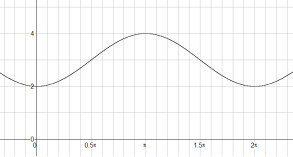
\includegraphics[ width=4.427in, height=2.3886in,]{L4SZ270G}
}


You would select the most appropriate way to tackle a problem based on the information given and the outcome expected. 

\subsubsection{Example}
Sketch $y =\cos  (x -\frac{\pi }{6})$ 

You could use a table of values however this is $y =\cos  x$ with a horizontal shift of $\frac{\pi }{6}$ to the right. 

Complete the following to show the answer. (This is the graph of $y =\cos  x .)$ 


\setlength\fboxrule{0.01in}\setlength\fboxsep{0.2in}\fcolorbox[HTML]{000000}{FFFFFF}{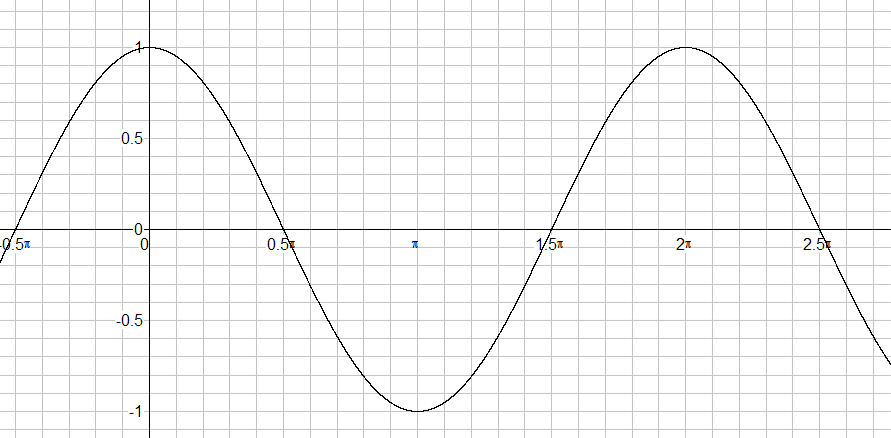
\includegraphics[ width=4.9095in, height=2.4275in,]{L4SZ270H}
}


\subsubsection{Example}
Sketch $y =2 \cos  t$ 


\begin{tabular}[c]{|l|l|l|l|l|l|}\hline
	$t$  & $0$  & $\frac{\pi }{2}$  & $\pi $  & $\frac{3 \pi }{2}$  & $2 \pi $  \\
	\hline
	$\cos  t$  & $1$  & $0$  & $ -1$  & $0$  & $1$  \\
	\hline
	$2 \cos  t$  & $2$  & $0$  & $ -2$  & $0$  & $2$  \\
	\hline
\end{tabular}

This is a vertical stretch of 2. You could roughly sketch this or use Desmos. 


\setlength\fboxrule{0.01in}\setlength\fboxsep{0.2in}\fcolorbox[HTML]{000000}{FFFFFF}{\includegraphics[ width=3.09in, height=2.0669in,]{L4SZ270I}
}


In general $y =a \sin  x$ represents a vertical stretch of $y =\sin  x$ by $a$. If $a$ is negative the transformation can either be described as a negative stretch or (preferably) as a \emph{stretch}
of $\left \vert a\right \vert $ followed by a \emph{reflection} in the $x$-axis. Recall the reflection of $y =f \left (x\right )$ in the $x$-axis is $y = -f \left (x\right )$. The number $\left \vert a\right \vert $ is called the \emph{amplitude} for both $y =\sin  x$ and $y =\cos  x\text{.}$ 

If $0 <a <1$ the fractional stretch causes the curve to shrink vertically. For instance the curve
$y =\sin  x$ has a maximum value of $1$ and a minimum value of $ -1$. the curve $y =\frac{1}{2} \sin  x$ has a maximum value of $\frac{1}{2}$ and a minimum value of $ -\frac{1}{2}$. 

\subsubsection{Example}
Sketch $y =\cos  ( -t)\text{.}$ 

Recall the reflection of $y =f (x)$in the $y$-axis is $y =f ( -x)$ so you would expect $y =\cos  ( -t)$ to be the reflection of $y =\cos  t$ in the $y$-axis. 


\begin{tabular}[c]{|l|l|l|l|l|l||l|l|l|l|l|l|l}
	$t$  & $0$  & $\frac{\pi }{2}$  & $\pi $  & $\frac{3 \pi }{2}$  & $2 \pi $  &  & $t$  & $0$  & $\frac{\pi }{2}$  & $\pi $  & $\frac{3 \pi }{2}$  & $2 \pi $  \\
	$ -t$  & $0$  & $ -\frac{\pi }{2}$  & $ -\pi $  & $ -\frac{3 \pi }{2}$  & $ -2 \pi $  &  & $\cos  t$  & $1$  & $0$  & $ -1$  & $0$  & $1$  \\
	$\cos  \left ( -t\right )$  & $1$  & $0$  & $ -1$  & $0$  & $1$  &  &  &  &  &  &  &  \\
	\multicolumn{1}{|l}{
	}
\end{tabular}

You can see from the table at the right that this looks exactly the same as
$y =\cos  t$ so $\cos  t$ is an \emph{even} function. When the $y$-axis is an axis of symmetry the function is an \emph{even} function. 


\setlength\fboxrule{0.01in}\setlength\fboxsep{0.2in}\fcolorbox[HTML]{000000}{FFFFFF}{\includegraphics[ width=4.587in, height=2.1689in,]{L4SZ270J}
}


\subsubsection{Example}
Sketch $y =\sin  \frac{1}{2} x$ 


\begin{tabular}[c]{|l|l|l|l|l|l|l|l|l|l|}\hline
	$x$  & $0$  & $\frac{\pi }{2}$  & $\pi $  & $\frac{3 \pi }{2}$  & $2 \pi $  & $\frac{5 \pi }{2}$  & $3 \pi $  & $\frac{7 \pi }{2}$  & $4 \pi $  \\
	\hline
	$\frac{1}{2} x$  & $0$  & $\frac{\pi }{4}$  & $\frac{\pi }{2}$  & $\frac{3 \pi }{4}$  & $\pi $  & $\frac{5 \pi }{4}$  & $\frac{3 \pi }{2}$  & $\frac{7 \pi }{4}$  & $2 \pi $  \\
	\hline
	$\sin  \frac{1}{2} x$  & $0$  &  & $1$  &  & $0$  &  & $ -1$  &  & $0$  \\
	\hline
\end{tabular}

In this case one cycle is achieved only after $x$ has reached $4 \pi $. The period therefore is $4 \pi $. 


\setlength\fboxrule{0.01in}\setlength\fboxsep{0.2in}\fcolorbox[HTML]{000000}{FFFFFF}{\includegraphics[ width=4.0698in, height=1.9372in,]{L4SZ270K}
}


\subsubsection{Example}
Sketch $y =\cos  2 x$ 


\begin{tabular}[c]{|l|l|l|l|l|l|}\hline
	$x$  & $0$  & $\frac{\pi }{2}$  & $\pi $  & $\frac{3 \pi }{2}$  & $2 \pi $  \\
	\hline
	$2 x$  & $0$  & $\pi $  & $2 \pi $  & $3 \pi $  & $4 \pi $  \\
	\hline
	$\cos  2 x$  & $1$  & $ -1$  & $1$  & $ -1$  & $1$  \\
	\hline
\end{tabular}

Maybe this is enough to enable you to sketch the curve. You notice the zeros that you usually get
in the table are missing and the way to include them is to select intermediate $x$ values. 


\begin{tabular}[c]{|l|l|l|l|l|l|}\hline
	$x$  & $0$  & $\frac{\pi }{4}$  & $\frac{\pi }{2}$  & $\frac{3 \pi }{4}$  & $\pi $  \\
	\hline
	$2 x$  & $0$  & $\frac{\pi }{2}$  & $\pi $  & $\frac{3 \pi }{2}$  & $2 \pi $  \\
	\hline
	$\cos  2 x$  & $1$  & $0$  & $ -1$  & $0$  & $1$  \\
	\hline
\end{tabular}


\setlength\fboxrule{0.01in}\setlength\fboxsep{0.2in}\fcolorbox[HTML]{000000}{FFFFFF}{\includegraphics[ width=3.0666in, height=1.9614in,]{L4SZ270L}
}


Notice by sketching from $0$ to $2 \pi $ $2$ cycles are drawn. The period here is $\pi $. There is a pattern emerging. Given
$y =\sin  k x$ or $y =\cos  k x$. The value of $k$ tells you how many cycles in $2 \pi $. If $k =2$ there are $2$ cycles in $2 \pi $ so one cycle takes $\pi $. If $k =\frac{1}{2}$ there is $\frac{1}{2}$ cycle in $2 \pi $ therefore one cycle will take $4 \pi $. Looking at this the other way. The
period is the interval required for one cycle so when $k =2$ the period $ =\pi $ and when $k =\frac{1}{2}$ the period $ =4 \pi \text{.}$ 

In general given $y =\sin  k x$ or $y =\cos  k x$ the period is $\frac{2 \pi }{k}$. 

In a test or exam, questions will be set to test these concepts, however, the topic can be complicated very
easily and in these cases Desmos or other software should be used to sketch the graph. 

\subsection{Exercises}
Graph the functions by hand. 

\begin{description}
	\item [1.]   
	%TCIMACRO{\TeXButton{Start Two Columns}{\columnsep =30pt
	% \begin {multicols}{2}}}%
	%BeginExpansion
	\columnsep =30pt
	\begin {multicols}{2}
	%EndExpansion
	$y =1 +\sin  x$ 
	
	\item [3.] $y =1 -\cos  x$ 
	%TCIMACRO{\TeXButton{End Two Columns}{\end {multicols}}}%
	%BeginExpansion
	\end {multicols}
	%EndExpansion
	
	\columnsep =30pt
	\begin {multicols}{2}
	\item [5.]
	%TCIMACRO{\TeXButton{Start Two Columns}{\columnsep =30pt
	% \begin {multicols}{2}}}%
	%BeginExpansion
	
	%EndExpansion
	$y = -2 \sin  x$ 
	
	\item [7.] $y =4 -2 \cos  x$ 
	%TCIMACRO{\TeXButton{End Two Columns}{\end {multicols}}}%
	%BeginExpansion
	\end {multicols}
	%EndExpansion
	
	
	\item [9.]
	$y =\left \vert \cos  x\right \vert $ \end{description}

Find the amplitude
and period of the function and sketch its graph. 


\begin{description}
	\item [11.]   
	%TCIMACRO{\TeXButton{Start Two Columns}{\columnsep =30pt
	% \begin {multicols}{2}}}%
	%BeginExpansion
	\columnsep =30pt
	\begin {multicols}{2}
	%EndExpansion
	$y =\cos  4 x$ 
	
	\item [13.] $y =3 \sin  3 x$ 
	%TCIMACRO{\TeXButton{End Two Columns}{\end {multicols}}}%
	%BeginExpansion
	\end {multicols}
	%EndExpansion
	
	
	\item [15.]
	%TCIMACRO{\TeXButton{Start Two Columns}{\columnsep =30pt
	% \begin {multicols}{2}}}%
	%BeginExpansion
	\columnsep =30pt
	\begin {multicols}{2}
	%EndExpansion
	$y =10 \sin  \frac{1}{2} x$ 
	
	\item [17.] $y = -\cos  \frac{1}{3} x$ 
	%TCIMACRO{\TeXButton{End Two Columns}{\end {multicols}}}%
	%BeginExpansion
	\end {multicols}
	%EndExpansion
	
	
	\item [19.]
	$y =3 \cos  3 \pi  x$ \end{description}

Find the amplitude, period and phase shift of the function,
and graph one complete period. 


\begin{description}
	\item [21.]   
	%TCIMACRO{\TeXButton{Start Two Columns}{\columnsep =30pt
	% \begin {multicols}{2}}}%
	%BeginExpansion
	\columnsep =30pt
	\begin {multicols}{2}
	%EndExpansion
	$y =\cos  \left (x -\frac{\pi }{2}\right )$ 
	
	\item [23.] $y = -\sin  \left (x -\frac{\pi }{6}\right )$ 
	%TCIMACRO{\TeXButton{End Two Columns}{\end {multicols}}}%
	%BeginExpansion
	\end {multicols}
	%EndExpansion
	
	
	\item [25.]
	%TCIMACRO{\TeXButton{Start Two Columns}{\columnsep =30pt
	% \begin {multicols}{2}}}%
	%BeginExpansion
	\columnsep =30pt
	\begin {multicols}{2}
	%EndExpansion
	$y =5 \cos  \left (3 x -\frac{\pi }{4}\right )$ 
	
	\item [27.] $y =2 \sin  \left (\frac{2}{3} x -\frac{\pi }{6}\right )$ 
	%TCIMACRO{\TeXButton{End Two Columns}{\end {multicols}}}%
	%BeginExpansion
	\end {multicols}
	%EndExpansion
	
	
	\item [29.]
	%TCIMACRO{\TeXButton{Start Two Columns}{\columnsep =30pt
	% \begin {multicols}{2}}}%
	%BeginExpansion
	\columnsep =30pt
	\begin {multicols}{2}
	%EndExpansion
	$y =3 \cos  \pi  \left (x +\frac{1}{2}\right )$ 
	
	\item [31.] $y = -\frac{1}{2} \cos  \left (2 x -\frac{\pi }{3}\right )$ 
	%TCIMACRO{\TeXButton{End Two Columns}{\end {multicols}}}%
	%BeginExpansion
	\end {multicols}
	%EndExpansion
	
	
	\item [33.]
	$y =\sin  \left (3 x +\pi \right )$ \end{description}

Use Desmos to complete the following questions: 

\begin{description}\item [41.]
	   
	%TCIMACRO{\TeXButton{Start Two Columns}{\columnsep =30pt
	% \begin {multicols}{2}}}%
	%BeginExpansion
	\columnsep =30pt
	\begin {multicols}{2}
	%EndExpansion
	$f (x) =\cos  100 x$ 
	
	\item [43.] $f (x) =\sin  \genfrac{(}{)}{}{}{x}{40}$ 
	%TCIMACRO{\TeXButton{End Two Columns}{\end {multicols}}}%
	%BeginExpansion
	\end {multicols}
	%EndExpansion
	
	
	\item [47.]
	$y =e^{\sin  20 x}$ \end{description}

Graph $f$, $g$ and $f +g$ on a common screen to illustrate graphical addition. 


\begin{description}
	\item [53.] $f \left (x\right ) =x\text{\quad \quad }g \left (x\right ) =\sin  x$ \end{description}

Graph the three functions on a common screen. How
are the graphs related? 


\begin{description}
	\item [55.]   
	%TCIMACRO{\TeXButton{Start Two Columns}{\columnsep =30pt
	% \begin {multicols}{2}}}%
	%BeginExpansion
	\columnsep =30pt
	\begin {multicols}{2}
	%EndExpansion
	$y =x^{2} ,\text{\quad \quad }y = -x^{2} ,\text{\quad \quad }y =x^{2} \sin  x$ 
	
	\item [57.] $y =e^{x} ,\text{\quad \quad }y = -e^{x} ,\text{\quad \quad }y =e^{x} \sin  5 \pi  x$ 
	%TCIMACRO{\TeXButton{End Two Columns}{\end {multicols}}}%
	%BeginExpansion
	\end {multicols}
	%EndExpansion
\end{description}

Find the maximum and minimum values of the function. 


\begin{description}
	\item [61.]   
	%TCIMACRO{\TeXButton{Start Two Columns}{\columnsep =30pt
	% \begin {multicols}{2}}}%
	%BeginExpansion
	\columnsep =30pt
	\begin {multicols}{2}
	%EndExpansion
	$y =\sin  x +\sin  2 x$ 
	
	\item [63.] $y =2 \sin  x +\sin ^{2} x$ 
	%TCIMACRO{\TeXButton{End Two Columns}{\end {multicols}}}%
	%BeginExpansion
	\end {multicols}
	%EndExpansion
\end{description}

Find all solutions of the equation that lie in the interval $\left [0 ,\pi \right ]$. State each answer
correct to 2 decimal places. 


\begin{description}
	\item [65.] $\cos  x =0.4$ \end{description}


%TCIMACRO{\TeXButton{Start Two Columns}{\columnsep =30pt
% \begin {multicols}{2}}}%
%BeginExpansion
\columnsep =30pt
\begin {multicols}{2}
%EndExpansion



%TCIMACRO{\TeXButton{End Two Columns}{\end {multicols}}}%
%BeginExpansion
\end {multicols}
%EndExpansion


\section{Trigonometric Graphs - Tangent}

This section in the textbook covers the tangent, cotangent, secant and cosecant functions. In
this course we will concentrate on the tangent function. the remaining three functions (often called the reciprocal
functions) will only be covered when they are needed. By focussing on sine, cosine and tangent the majority
of problems we encounter can be solved. Furthermore these are the functions we can evaluate immediately by pressing
appropriate keys on the calculator. 

Previously we learnt that the period for the sine and cosine functions was $2 \pi $. Tangent is also a periodic function and it has a period of $\pi $ (not $2 \pi $). This means that it goes through one complete cycle every $2 \pi $. Recall $\tan  t =\frac{\sin  t}{\cos  t}$. To analyse the behaviour of the tangent function it helps if you know what you are looking
for. You should know the shape of $y =\tan  t$ from previous courses. Some key values of tangent will show the pattern. 


\begin{tabular}[c]{|l|l|l|l|}\hline
	$t$  & $\sin  t$  & $\cos  t$  & $\tan  t$  \\
	\hline
	$ -\frac{\pi }{2}$  & $ -1$  & $0$  & $\frac{ -1}{0} = -\infty $  \\
	\hline
	$ -\frac{\pi }{4}$  & $ -\frac{\sqrt{2}}{2}$  & $\frac{\sqrt{2}}{2}$  & $ -\frac{\sqrt{2}}{2} \div \frac{\sqrt{2}}{2} = -1$  \\
	\hline
	$0$  & $0$  & $1$  & $\frac{0}{1} =0$  \\
	\hline
	$\frac{\pi }{4}$  & $\frac{\sqrt{2}}{2}$  & $\frac{\sqrt{2}}{2}$  & $\frac{\sqrt{2}}{2} \div \frac{\sqrt{2}}{2} =1$  \\
	\hline
	$\frac{\pi }{2}$  & $1$  & $0$  & $\frac{1}{0} =\infty $  \\
	\hline
\end{tabular}

As $t$ takes values from $ -\frac{\pi }{2}$ to $\frac{\pi }{2}$, $\tan  t$ takes values from $ -\infty $ to $\infty $. This pattern is repeated every $\pi $. Mathematically we say
\begin{equation*}\tan  \left (t +n \pi \right ) =\tan  t\text{\  } \forall n \in \mathbb{Z}
\end{equation*}

Furthermore $y =\tan  t$ is an \emph{odd function} so
\begin{equation*}\tan  \left ( -t\right ) = -\tan  t
\end{equation*}

An Desmos graph can show this relationship 


\setlength\fboxrule{0.01in}\setlength\fboxsep{0.2in}\fcolorbox[HTML]{000000}{FFFFFF}{\includegraphics[ width=5.9646in, height=2.8772in,]{L4SZ270M}
}


The graph can be seen to have point symmetry. If you rotate the tangent curve through
a half turn using the origin as axis the curve will lie on top of itself. This is a pictorial representation
of an odd function.

Aside: You must not confuse $y =\tan  x$ with $y =x^{3}$. While they may appear to be similar in shape the only similarities are that they both
pass through the origin and continue towards $\infty $ in the first quadrant and $ -\infty $ in the third quadrant. Important differences that you should identify if you
are asked to sketch these graphs are the slope of the curves at the origin and the behaviour as $y \leadsto  \pm \infty $. 


\begin{tabular}[c]{l|l|l|}  & $y =x^{3}$  & $y =\tan  x$  \\
	\hline
	Slope of the curve at the origin  & $m =0$ {\scriptsize (horizontal)}  & $m =1$  \\
	\hline
	As $y \leadsto \infty $  & As $x \leadsto \infty $ $y \leadsto \infty $  & As $x \leadsto \frac{\pi }{2}$ $y \leadsto \infty $  \\
	\hline
	As $y \leadsto  -\infty $  & As $x \leadsto  -\infty $ $y \leadsto  -\infty $  & As $x \leadsto  -\frac{\pi }{2}$ $y \leadsto  -\infty $  \\
	\hline
	Asymptotes  & No
	asymptotes  & Every $\left (2 n -1\right ) \frac{\pi }{2}$ $\left ( \forall n \in \mathbb{Z}\right )$  \\
	\hline
	Periodicity
	& No period  & Period $ =\pi $  \\
	\hline
	Domain  & $\mathbb{R}$  & $\mathbb{R}$ except $\left (2 n -1\right ) \frac{\pi }{2}$  \\
	\hline
\end{tabular}

%\subsection{Transformations}
%The six transformations that we reviewed in section 7.3 apply also to the tangent function. 
%
%\subsubsection{Example}
%(a) $y =\tan  \left (x -2\right )$ shifts the tangent curve 2 to the right. 
%
%(b) $y =\tan  x +2$ shifts the tangent curve 2 upwards. 
%
%(c) $y =2 \tan  x$ is a vertical stretch of $2$. 
%
%(d) $y =\tan  2 x$ is a horizontal stretch of $\frac{1}{2}$. 
%
%(e) $y = -\tan  x$ is a reflection in the $x$-axis. 
%
%(f) $y =\tan  \left ( -x\right )$ is a reflection in the $y$-axis. 
%
%You could use Desmos to verify that these are correctly stated. 
%
%$y =a \tan  k t$ where $a$ and $k$ are both $ >0$ represent a vertical stretch of $a$ and a horizontal stretch of $\frac{1}{k}$. This means that if the period of $y =\tan  t$ is $\pi $ then the period of $y =a \tan  k t$ is $\frac{\pi }{k}$. If $0 <a <1$ the transformation is a shrinking not a stretching. If $0 <k <1$ then $\frac{1}{k} >1$. The period (which is $\frac{\pi }{k} =\pi  \times \frac{1}{k}$) will be $ >\pi $. 

\subsection{Exercises}

\begin{description}
	\item [1.] A point $P ( -\frac{\sqrt{3}}{2} ,\frac{1}{2})$ is given. (a) Show that $P$ lies on the unit circle. (b) Suppose that $P$ is the terminal point determined by $t$. Find $\sin  t$, $\cos  t$ and $\tan  t\text{.}$ 
	
	\item [3.] Given $t =\frac{2 \pi }{3}\text{.}$ Find the terminal point $P (x ,y)$ on the unit circle determined by $t$ and find $\sin  t$, $\cos  t$ and $\tan  t\text{.}$ \end{description}

Find the values of the trigonometric ratios.
\ If possible give the exact value; otherwise use a calculator to find an approximate value correct to 5 decimal
places. 


\begin{description}
	\columnsep =30pt
\begin {multicols}{2}
	\item [9.]   
	%TCIMACRO{\TeXButton{Start Two Columns}{\columnsep =30pt
	% \begin {multicols}{2}}}%
	%BeginExpansion
	%EndExpansion
	(a) $\sin  1.1\text{\quad \quad }$(b) $\cos  1.1$ 
	
	\item [10.] (a) $\cos  \frac{\pi }{5}\text{\quad \quad }$(b) $\cos  \left ( -\frac{\pi }{5}\right )$ 
	%TCIMACRO{\TeXButton{End Two Columns}{\end {multicols}}}%
	%BeginExpansion
	\end {multicols}
	%EndExpansion
	
	
	\item [21.]
	Given $\sin  t =\frac{5}{13}$ and $\cos  t = -\frac{12}{13}$ find $\tan  t$ \end{description}

\section{Answers}
\textbf{Exercises} 

\begin {multicols}{2}

5. $P \left (\frac{4}{5} ,\frac{3}{5}\right )$ 

7. $P \left (\frac{ -\sqrt{5}}{3} ,\frac{2}{3}\right )$ 

9. $P \left (\frac{ -\sqrt{2}}{3} ,\frac{ -\sqrt{7}}{3}\right )$ 

13. $\left (0 ,1\right )$ 

15. $\left (\frac{ -\sqrt{3}}{2} ,\frac{1}{2}\right )$ 

17. $\left (\frac{1}{2} ,\frac{ -\sqrt{3}}{2}\right )$ 

19. $\left ( -\frac{1}{2} ,\frac{\sqrt{3}}{2}\right )$ 

21. $\left (\frac{ -\sqrt{2}}{2} ,\frac{ -\sqrt{2}}{2}\right )$ 

23. (a) $\left ( -\frac{3}{5} ,\frac{4}{5}\right )$, (b) $\left (\frac{3}{5} , -\frac{4}{5}\right )$ (c) $\left ( -\frac{3}{5} , -\frac{4}{5}\right )$  \\\relax (d)
$\left ( -\frac{3}{5} , -\frac{4}{5}\right )$ 

\end{multicols}

\textbf{Exercises} 
\begin{multicols}{2}

3.
(a) $\frac{ -\sqrt{3}}{2}$ (b) $\frac{1}{2}$ 

5. (a) $ -1$ (b) $ -1$ 

7. (a) $1$ (b) $ -1$ 

9. (a) $0$ (b) $0$ 

13. (a) $\frac{1}{2}$ (b) $\frac{1}{2}$ 

15. (a) $\frac{\sqrt{3}}{3}$ (b) $\frac{ -\sqrt{3}}{3}$ 

27. $\frac{4}{5} ,\frac{3}{5} ,\frac{4}{3}$ 

29. $\frac{ -\sqrt{11}}{4} ,\frac{\sqrt{5}}{4} ,\frac{ -\sqrt{55}}{5}$ 

35. $0.84147$ 

37. $0.93204$ 

39. $1.02964$ 

41. $ -0.57482\vspace{+5.000000cm}$ 
\end{multicols}
\clearpage

\textbf{Exercises} 
\begin{multicols}{2}

\begin{tabular}[c]{ll}1.  &
	\setlength\fboxrule{0.01in}\setlength\fboxsep{0.2in}\fcolorbox[HTML]{000000}{FFFFFF}{\includegraphics[ width=1.7115in, height=0.9625in,]{L4SZ270N}
	}
	\vspace{0.5cm}  \\
	3.  &
	\setlength\fboxrule{0.01in}\setlength\fboxsep{0.2in}\fcolorbox[HTML]{000000}{FFFFFF}{\includegraphics[ width=1.7279in, height=0.9945in,]{L4SZ270O}
	}
	\vspace{0.5cm}  \\
	5.  &
	\setlength\fboxrule{0.01in}\setlength\fboxsep{0.2in}\fcolorbox[HTML]{000000}{FFFFFF}{\includegraphics[ width=1.7253in, height=1.7737in,]{L4SZ270P}
	}
	\vspace{0.5cm}  \\
	7.  &
	\setlength\fboxrule{0.01in}\setlength\fboxsep{0.2in}\fcolorbox[HTML]{000000}{FFFFFF}{\includegraphics[ width=1.753in, height=1.1727in,]{L4SZ270Q}
	}
	\vspace{0.5cm}  \\
	9.  &
	\setlength\fboxrule{0.01in}\setlength\fboxsep{0.2in}\fcolorbox[HTML]{000000}{FFFFFF}{\includegraphics[ width=1.7642in, height=0.9167in,]{L4SZ270R}
	}
	\vspace{0.5cm}
\end{tabular}


\begin{tabular}[c]{ll}11.  & $1 ,\frac{\pi }{2}$  \\
	&    
	\setlength\fboxrule{0.01in}\setlength\fboxsep{0.2in}\fcolorbox[HTML]{000000}{FFFFFF}{\includegraphics[ width=1.9666in, height=1.4157in,]{L4SZ270S}
	}
\end{tabular}


\begin{tabular}[c]{ll}13.  & $3 ,\frac{2 \pi }{3}$  \\
	&    
	\setlength\fboxrule{0.01in}\setlength\fboxsep{0.2in}\fcolorbox[HTML]{000000}{FFFFFF}{\includegraphics[ width=1.9692in, height=1.3569in,]{L4SZ270T}
	}
\end{tabular}


\begin{tabular}[c]{ll}15.  & $10 ,4 \pi $  \\
	&    
	\setlength\fboxrule{0.01in}\setlength\fboxsep{0.2in}\fcolorbox[HTML]{000000}{FFFFFF}{\includegraphics[ width=2.1802in, height=1.1744in,]{L4SZ270U}
	}
\end{tabular}


\begin{tabular}[c]{ll}17.  & $1 ,6 \pi $  \\
	&    
	\setlength\fboxrule{0.01in}\setlength\fboxsep{0.2in}\fcolorbox[HTML]{000000}{FFFFFF}{\includegraphics[ width=2.3013in, height=1.036in,]{L4SZ270V}
	}
\end{tabular}


\begin{tabular}[c]{ll}19.  & $3 ,\frac{2}{3}$ note the non-trig scale  \\
	&
	\setlength\fboxrule{0.01in}\setlength\fboxsep{0.2in}\fcolorbox[HTML]{000000}{FFFFFF}{\includegraphics[ width=2.4933in, height=1.4806in,]{L4SZ270W}
	}
\end{tabular}


\begin{tabular}[c]{ll}21.  & $1 ,2 \pi  ,\frac{\pi }{2}$  \\
	&    
	\setlength\fboxrule{0.01in}\setlength\fboxsep{0.2in}\fcolorbox[HTML]{000000}{FFFFFF}{\includegraphics[ width=2.4794in, height=1.4416in,]{L4SZ270X}
	}
\end{tabular}


\begin{tabular}[c]{ll}23.  & $2 ,2 \pi  ,\frac{\pi }{6}$  \\
	&    
	\setlength\fboxrule{0.01in}\setlength\fboxsep{0.2in}\fcolorbox[HTML]{000000}{FFFFFF}{\includegraphics[ width=2.4794in, height=1.4883in,]{L4SZ270Y}
	}
\end{tabular}


\begin{tabular}[c]{ll}25.  & $5 ,\frac{2 \pi }{3} ,\frac{\pi }{12}$  \\
	&    
	\setlength\fboxrule{0.01in}\setlength\fboxsep{0.2in}\fcolorbox[HTML]{000000}{FFFFFF}{\includegraphics[ width=2.1724in, height=1.9441in,]{L4SZ270Z}
	}
\end{tabular}


\begin{tabular}[c]{ll}27.  & $2 ,3 \pi  ,\frac{\pi }{4}$  \\
	&    
	\setlength\fboxrule{0.01in}\setlength\fboxsep{0.2in}\fcolorbox[HTML]{000000}{FFFFFF}{\includegraphics[ width=2.4336in, height=1.1243in,]{L4SZ2710}
	}
\end{tabular}


\begin{tabular}[c]{ll}29.  & $3 ,2 , -\frac{1}{2}$  \\
	&    
	\setlength\fboxrule{0.01in}\setlength\fboxsep{0.2in}\fcolorbox[HTML]{000000}{FFFFFF}{\includegraphics[ width=2.1543in, height=1.8498in,]{L4SZ2711}
	}
\end{tabular}


\begin{tabular}[c]{ll}31.  & $\frac{1}{2} ,\pi  ,\frac{\pi }{6}$  \\
	&    
	\setlength\fboxrule{0.01in}\setlength\fboxsep{0.2in}\fcolorbox[HTML]{000000}{FFFFFF}{\includegraphics[ width=1.9216in, height=1.4797in,]{L4SZ2712}
	}
\end{tabular}


\begin{tabular}[c]{ll}33.  & $1 ,\frac{2 \pi }{3} , -\frac{\pi }{3}$  \\
	&    
	\setlength\fboxrule{0.01in}\setlength\fboxsep{0.2in}\fcolorbox[HTML]{000000}{FFFFFF}{\includegraphics[ width=1.4408in, height=1.6397in,]{L4SZ2713}
	}
\end{tabular}


\begin{tabular}[c]{ll}41.  &  \\
	&
	\setlength\fboxrule{0.01in}\setlength\fboxsep{0.2in}\fcolorbox[HTML]{000000}{FFFFFF}{\includegraphics[ width=2.3168in, height=1.2315in,]{L4SZ2714}
	}
\end{tabular}


\begin{tabular}[c]{ll}43.  &  \\
	&
	\setlength\fboxrule{0.01in}\setlength\fboxsep{0.2in}\fcolorbox[HTML]{000000}{FFFFFF}{\includegraphics[ width=2.0989in, height=1.3214in,]{L4SZ2715}
	}
\end{tabular}


\begin{tabular}[c]{ll}47.  &  \\
	&
	\setlength\fboxrule{0.01in}\setlength\fboxsep{0.2in}\fcolorbox[HTML]{000000}{FFFFFF}{\includegraphics[ width=2.3722in, height=1.3872in,]{L4SZ2816}
	}
\end{tabular}


\begin{tabular}[c]{ll}53.  &  \\
	&
	\setlength\fboxrule{0.01in}\setlength\fboxsep{0.2in}\fcolorbox[HTML]{000000}{FFFFFF}{\includegraphics[ width=2.4621in, height=2.2096in,]{L4SZ2817}
	}
\end{tabular}


\begin{tabular}[c]{ll}55.  &  \\
	&
	\setlength\fboxrule{0.01in}\setlength\fboxsep{0.2in}\fcolorbox[HTML]{000000}{FFFFFF}{\includegraphics[ width=2.5399in, height=1.3085in,]{L4SZ2818}
	}
\end{tabular}


\begin{tabular}[c]{ll}57.  &  \\
	&
	\setlength\fboxrule{0.01in}\setlength\fboxsep{0.2in}\fcolorbox[HTML]{000000}{FFFFFF}{\includegraphics[ width=2.5564in, height=1.6371in,]{L4SZ2819}
	}
\end{tabular}
\end{multicols}

61. Maximum value $1.76$ when $x \approx 0.94$, minimum value $ -1.76$ when $x \approx  -0.94\text{.}$ The same maximum and minimum values occur at infinitely many other values
of $x$. 

63. Maximum value $3.00$ when $x \approx 1.57\text{,}$ minimum value $ -1.00$ when $x \approx  -1.57$. The same maximum and minimum values occur at infinitely many other values of $x$. 

65. $1.16$ 

\textbf{Exercises} 
\begin{multicols}{2}

1. (b) $\frac{1}{2} ,\frac{ -\sqrt{3}}{2} ,\frac{ -\sqrt{3}}{3}$ 

3. $\left ( -\frac{1}{2} ,\frac{\sqrt{3}}{2}\right ) ,\sin  t =\frac{\sqrt{3}}{2} ,\cos  t = -\frac{1}{2} ,\tan  t = -\sqrt{3}$ 

9. (a) $0.89121$ (b) $0.45360$ 

10. (a) $0.80902$ (b) $0.80902$ 

21. $ -\frac{5}{12}$ 
\end{multicols}

